% (c)~2014 Dimitrios Vrettos - d.vrettos@gmail.com
% (c)~2014 Claudio Carboncini - claudio.carboncini@gmail.com
% (c)~2015 Daniele Zambelli daniele.zambelli@gmail.com
% (c)~2015 Maria Antonietta Pollini

% \begin{inaccessibleblock}[?.]
% \centering
%   \input{\folder lbr/?.pgf}
%   \caption{?.} \label{fig:?_?}
% \end{inaccessibleblock}

% \begin{figure}[h]
% \begin{minipage}{.40\textwidth}
% 
% \end{minipage}
% \begin{minipage}{.60\textwidth}
% \begin{inaccessibleblock}[?]
% \centering
%   \input{\folder lbr/?.pgf}
%   \caption{?.} \label{fig:?_?}
% \end{inaccessibleblock}
% \end{minipage}
% \end{figure}

% \begin{wrapfloat}{figure}{r}{0pt}
% \includegraphics[scale=0.35]{img/?.png}
% \caption{?}
% \label{fig:?_?}
% \end{wrapfloat}
% 
% \begin{center} \input{\folder lbr/?.pgf} \end{center}

\begin{comment}
 
 \begin{minipage}{.45\textwidth}
  
 \end{minipage}
 \begin{minipage}{.25\textwidth}
  
 \end{minipage}
 \begin{minipage}{.3\textwidth}
  
 \end{minipage}
 
\end{comment}

\chapter{Disequazioni}

\section{Risoluzione delle disequazioni di secondo grado}
\label{sec:diseq_secondo_grado}

Una disequazione di secondo grado si presenta in una delle seguenti forme:
\[ax^2+bx+c<0;\quad ax^2+bx+c\le 0;\quad ax^2+bx+c\ge0;\quad ax^2+bx+c> 0\]

Ricordiamo che risolvere una disequazione in un'incognita significa determinare 
l'insieme dei valori da attribuire all'incognita affinché la disequazione sia 
verificata.
Abbiamo già imparato che per risolvere una disequazione di primo grado dobbiamo 
studiare il segno del binomio di primo grado, così, per risolvere una 
disequazione di secondo grado dobbiamo studiare il segno di un polinomio di 
secondo grado.

\subsection{Studio del segno di un trinomio di secondo grado}
\label{sec:diseq_trinomio}

Studiare il segno di un polinomio vuol dire stabilire per quali valori 
di~$x$ esso assume segno positivo, per quali segno negativo e per quali 
si annulla.

Ricordiamo che un polinomio in una sola variabile, solitamente indicata con 
$x$, 
è di secondo grado se il massimo esponente della variabile è $2$. 
Per \emph{trinomio di secondo grado} intendiamo un polinomio di secondo grado: 
$ax^2+bx+c$ con $a\in \insR_{0},~b\in \insR,~c\in \insR$. 
Chiamiamo \emph{zeri del trinomio} i numeri reali soluzione dell'equazione 
associata al polinomio: $ax^2+bx+c=0$.

\begin{definizione}
Una \emph{funzione polinomiale di secondo grado} è una funzione che associa ad 
ogni numero reale $x$ il numero reale $y$ tale che
$y=ax^2+bx+c$ con $a\in \insR_{0}$, $b\in \insR$, $c\in \insR$.
\end{definizione}

Nel riferimento cartesiano ortogonale il grafico della funzione è costituito da 
tutti e soli i punti le cui coordinate soddisfano l'equazione $y=ax^2+bx+c$ se 
$x_1$ e $x_2$ sono gli zeri reali del trinomio $ax^2+bx+c$ allora attribuendo 
tali valori alla variabile $x$ si ha $y=0$ essi sono dunque \emph{gli zeri 
della 
funzione}, ossia le ascisse dei punti del grafico appartenenti all'asse $x$.

Assegnata la funzione polinomiale di secondo grado $y={ax}^2+{bx}+c$ con 
$a\neq 0$, sappiamo che il grafico di tale curva è una parabola. 
In particolare:
\begin{itemize*}
\item il coefficiente $a$ indica la concavità: verso l'alto se $a>0$, verso il 
basso se $a<0$
\item il coefficiente $c$ indica l'intersezione della parabola con l'asse delle 
$y$
\item dalle formule $-2av_x=b$ e $a(v_x)^2+v_y=c$ ricaviamo le coordinate del 
suo vertice:
\[v_x=-\frac b{2a} \text{ e } 
  v_y=c-a\left(-\frac{b}{2a}\right)^2=\frac{4ac-b^2}{4a}=-\frac{\Delta }{4a}\]
\item risolvendo l'equazione ${ax}^2+{bx}+c=0$ determiniamo gli eventuali punti 
di intersezione con l'asse $x$ (gli zeri della funzione).
\end{itemize*}

% \begin{exrig}
\begin{esempio}
Data la funzione $f: y=x^2-2x-3$ tracciare nel riferimento cartesiano 
ortogonale 
il suo grafico.
Il grafico di tale curva è una parabola:
\begin{itemize*}
\item essendo il coefficiente $a=1$, la concavità è verso l'alto;
\item il coefficiente $c=-3$ corrisponde al punto $P(0,-3)$ in cui la parabola 
incontra l'asse delle $y$
\item essendo $ a=1 $, $b=-2$ e $c=-3$ le coordinate del vertice sono 
$v_x=-\frac{-2} 2=1$ e $v_y=\frac{-12-4} 4=-4$
\item le ascisse dei punti $(-1;0)$ e $(3;0)$ rappresentano gli zeri della 
funzione, soluzione dell'equazione $x^2-2x-3=0$
\item altri punti della parabola si trovano assegnando alla variabile 
indipendente valori arbitrari: per $x=2$ otteniamo $y=(2)^2-2(2)-3=-3$, il 
punto 
$P(2;-3)$ è un punto della parabola.
\end{itemize*}

\begin{center}
 % (c) 2013 Claudio Carboncini - claudio.carboncini@gmail.com
% (c) 2014 Dimitrios Vrettos - d.vrettos@gmail.com
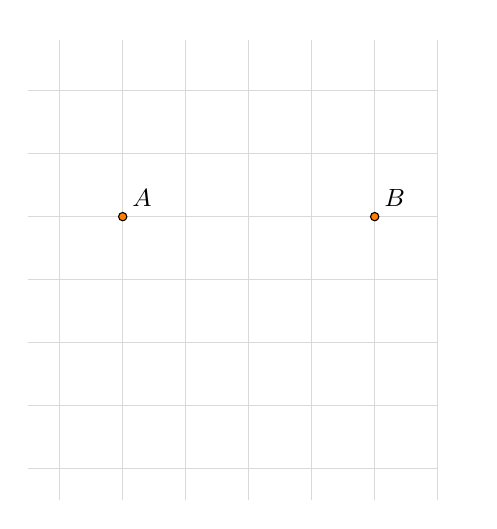
\begin{tikzpicture}[x=8mm, y=8mm,font=\small]

  \node[above right] at (-1,0) {$A$};
  \node[above right] at (3,0) {$B$};
  \draw[step=0.8cm,color=gray!30] (-2.5,-4.5) grid (4,2.8);
  \tkzInit[xmin=-2,xmax=3.5,ymin=-4.5,ymax=2]
  \clip (-2.5,-4.3) rectangle (4.5,3);
  \begin{scope}[font=\small]
    \tkzAxeY[orig = false, label options={left = 1pt}]
    \tkzAxeX[orig = true, label options={below = 1pt}]
  \end{scope}
  \tkzFct[domain=-1.3:3.3,thick,color=Maroon]{x*x-2*x-3};
  \draw[fill=orange] (-1,0)circle (1.5pt);
  \draw[fill=orange] (3,0)circle (1.5pt);

\end{tikzpicture}

\end{center}
\end{esempio}
\begin{esempio}
Studiare il segno del trinomio $x^2-2x-3$.

La richiesta è interpretabile anche come la ricerca degli insiemi soluzione 
dell'equazione $x^2-2x-3=0$ e delle disequazioni $x^2-2x-3>0$ e $x^2-2x-3<0$.

\emph{Strategia risolutiva}:
Tracciamo il grafico della funzione $y=x^2-2x-3$ e leggiamo dal grafico gli 
insiemi richiesti (vedi figura precedente):
\begin{itemize*}
\item I valori di~$x$ che rendono l'ordinata nulla sono le ascisse dei punti~A 
e~B e costituiscono l'insieme soluzione dell'equazione $x^2-2x-3=0$ cioè 
$x_1=-1\vee x_2=3$
\item I valori di $x$ dell'insieme $H=\{x\in \insR | x_A<x<x_B\}$ rendono il 
trinomio negativo; infatti preso un valore dell'insieme, ad esempio $x=0$, il 
punto sulla parabola ha ordinata negativa $(-3)$. Segnatelo sul grafico accanto 
e ripetete per $x=1$, $x=\frac 3 2$, $x=2$.
I valori dell'insieme H sono le soluzioni della disequazione $x^2-2x-3<0$.
\item I valori di $x$ dell'insieme $K=\{x\in \insR | x<x_A\vee x>x_B\}$ rendono 
il trinomio positivo; infatti preso un valore dell'insieme, ad esempio $x=\frac 
7 2$, il punto sulla parabola ha ordinata positiva. Segnatelo sul grafico 
accanto e ripetete per $x=-\frac{6}{5}$.
I valori dell'insieme K sono interpretabili come le soluzioni della 
disequazione 
$x^2-2x-3>0$.
\end{itemize*}
\end{esempio}
% \end{exrig}

\osservazione La ricerca dell'insieme soluzione di una disequazione di secondo 
grado è sempre interpretabile come la ricerca del segno di un trinomio di 
secondo grado e quindi risolubile per via grafica. In questi casi non è 
necessario rappresentare in modo preciso la parabola associata al trinomio, ma 
basta ricordare quanto detto inizialmente sugli zeri di una funzione.

% \begin{exrig}
\begin{esempio}
Risolvi le seguente disequazioni utilizzando lo studio del segno del trinomio 
di secondo grado.

%%%%%%%%%%%%%%%%%%%%%% Usare lo schema già utilizzato per il primo grado


\begin{itemize}
\item $x^2+x-2>0$.

Risolviamo l'equazione associata $x^2+x-2=0$ che avendo il discriminante 
positivo $b^2-4ac=9>0$ ammette due soluzioni reali distinte $x_1=-2\vee x_2=1$. 
I due numeri $1$ e $-2$ sono gli zeri del trinomio e dunque gli zeri della 
funzione $y=x^2+x-2$. La parabola $y=x^2+x-2$ volge la concavità verso l'alto, 
essendo $a=1>0$, quindi possiamo grossolanamente rappresentare la sua 
posizione rispetto all'asse x come in figura.
Le ascisse dei punti esterni ai due punti di intersezione con l'asse delle x 
rendono il segno del trinomio positivo, perché corrispondono a punti del 
grafico 
le cui ordinate sono positive.  L'insieme soluzione della disequazione 
$x^2+x-2>0$ è dato da: $\IS=\{x\in \insR\text{{\textbar} }x<-2\vee x>1\}$ o con 
notazione insiemistica $(-\infty,-2)\cup (1,+\infty )$

\item $x^2-4x+4\le 0$.

Risolviamo l'equazione associata $x^2-4x+4=0$ che avendo il discriminante nullo 
ammette due soluzioni reali coincidenti $x_1=x_2=2$: gli zeri del trinomio sono 
coincidenti nel numero $2$. La parabola $y=x^2-4x+4$ ha il vertice sull'asse 
$x$ 
e volge la concavità verso l'alto quindi possiamo grossolanamente rappresentare 
la sua posizione come in figura.Tutti i punti del grafico hanno ordinata 
positiva, eccetto 
quello di intersezione con l'asse~x, che ha ordinata nulla.. Nessun valore 
reale rende pertanto il trinomio negativo; $x=2$ lo rende nullo.L'insieme 
soluzione richiesto: $\IS=\{x\in \insR\text{{\textbar} }x=2\}$.;

\item $x^2-2x+7>0$.

Risolviamo l'equazione associata $x^2-2x+7=0$ che avendo il discriminante 
negativo non ammette soluzioni reali; il trinomio non ha zeri reali, la 
parabola 
$y=x^2-2x+7$ volge la concavità  verso l'alto e non ha punti appartenenti 
all'asse $x$ quindi possiamo grossolanamente rappresentare la sua posizione  
come in figura. Tutti i punti del grafico hanno ordinata positiva. Pertanto 
l'insieme soluzione della disequazione data è: $\IS=\insR$.
\end{itemize}
\begin{center}
 % (c) 2013 Claudio Carboncini - claudio.carboncini@gmail.com
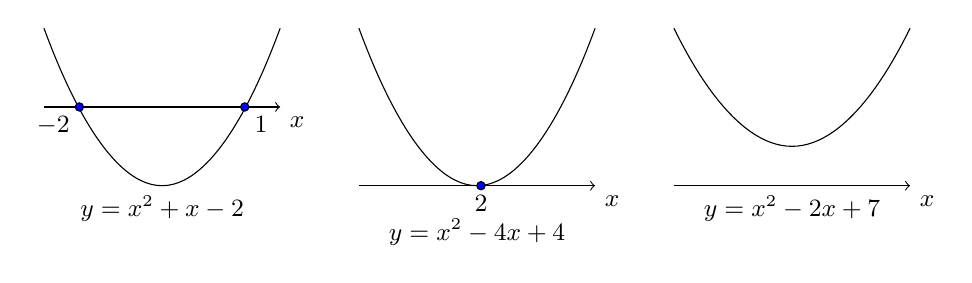
\begin{tikzpicture}[font=\small,x=10mm, y=10mm]
% prima parabola;
  \draw (-1,0) parabola[parabola height=-2cm] +(3,0);
  \draw[->] (-1,-1) -- (2,-1) node [below right] () {$x$};
  \draw[fill=blue] (-.55,-1)circle (1.5pt);
  \draw[fill=blue] (1.55,-1)circle (1.5pt);
  \node[below left] at (-.55,-1) {$-2$};
  \node[below right] at (1.55,-1) {$1$};
  \node[below] at(.5,-2) {$y=x^2+x-2$};
%seconda parabola
  \draw (3,0) parabola[parabola height=-2cm] +(3,0);
  \draw[->] (3,-2) -- (6,-2) node [below right] () {$x$};
  \draw[fill=blue] (4.55,-2)circle (1.5pt);
  \node[below] at (4.55,-2) {$2$};
  \node[below] at(4.5,-2.3) {$y=x^2-4x+4$};
 % terza parabola;
  \draw (7,0) parabola[parabola height=-1.5cm] +(3,0);
  \draw[->] (7,-2) -- (10,-2) node [below right] () {$x$};
  \node[below] at(8.5,-2) {$y=x^2-2x+7$};
\end{tikzpicture}


\end{center}
\end{esempio}

% % \end{exrig}
% \vspazio\ovalbox{\risolvii \ref{ese:4.9}, \ref{ese:4.10}, \ref{ese:4.11}, 
% \ref{ese:4.12}, \ref{ese:4.13}, \ref{ese:4.14}, \ref{ese:4.15}, 
% \ref{ese:4.16}, 
% \ref{ese:4.17}, \ref{ese:4.18}, \ref{ese:4.19}, \ref{ese:4.20}, 
% \ref{ese:4.21},}
% 
% \vspazio\ovalbox{ \ref{ese:4.22}, \ref{ese:4.23}, \ref{ese:4.24}, 
% \ref{ese:4.25}, \ref{ese:4.26}}
% 
% 
% %%%%%%%%%%%%%%%%%%%%%%%%%%%%%%
% % \begin{exrig}

\begin{esempio}
Determinare l'insieme soluzione della disequazione $2x^2-5\le 0$.

L'equazione associata $2x^2-5=0$ è pura con soluzioni reali $x=\pm \sqrt{\frac 
5 2}$. Razionalizzando otteniamo: $x_1=-\frac{\sqrt{10}} 2\vee 
x_2=+\frac{\sqrt{10}} 2$. La parabola associata $y=2x^2-5$ interseca quindi 
l'asse delle x in due punti, rispettivamente di ascisse 
$x_1=-\frac{\sqrt{10}} 2\vee x_2=+\frac{\sqrt{10}} 2$ 
e ha concavità rivolta verso l'alto, essendo il coefficiente~$a$ uguale a~$+2$.
Riporta qui a lato la configurazione della parabola.
Da essa puoi osservare che i punti del grafico con ordinata negativa o nulla 
sono quelli la cui ascissa è compresa fra le ascisse dei due punti di 
intersezione con l'asse delle x o è ad essa uguale.L'insieme soluzione della 
disequazione data 
 $\IS=\left\{x\in \insR | -\frac{\sqrt{10}} 2\le x\le +\frac{\sqrt{10}} 
2\right\}$.
\end{esempio}


\begin{esempio}
Determinare l'insieme soluzione della disequazione $-3x^2+2x>0$.

L'equazione associata è $-3x^2+2x=0$ con le radici $x_1=0\vee x_2=\frac 2 3$. 
La parabola associata $y=-3x^2+2x$ interseca l'asse delle x in due punti, 
rispettivamente di ascisse $x_1=0\vee x_2=\frac 2 3$ e ha concavità rivolta 
verso il basso, essendo il coefficiente a uguale a -3.Riporta qui a lato la 
configurazione della parabola.
Da essa puoi osservare che i punti del grafico con ordinata positiva sono 
quelli 
la cui ascissa è compresa fra le ascisse dei due punti di intersezione con 
l'asse delle x.
Pertanto la disequazione assegnata ha $\IS=\left\{x\in \insR | 0<x<\frac 2 
3\right\}$.
\end{esempio}

% \end{exrig}

Si riporta di seguito la classificazione delle diverse 
tipologie di disequazione di secondo grado con le relative rappresentazioni 
grafiche e soluzioni.

% \begin{inaccessibleblock}[I sei casi di posizione di una parabola rispetto 
%   all'asse~x.]
%  \begin{figure}[tp]
% \centering
% % (c) 2013 Claudio Carboncini - claudio.carboncini@gmail.com
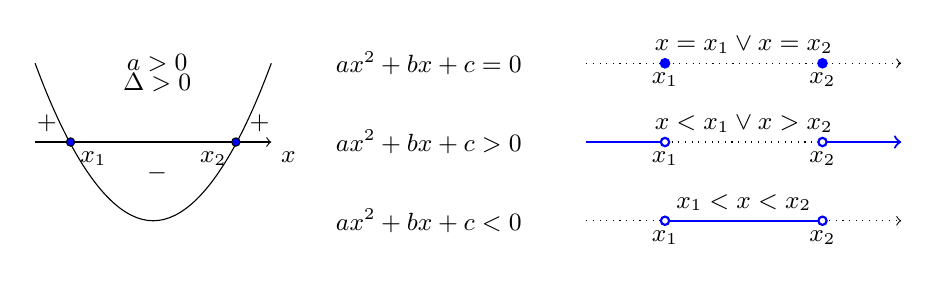
\begin{tikzpicture}[font=\small,x=10mm, y=10mm]

% prima parabola;
  \draw (-1,0) parabola[parabola height=-2cm] +(3,0);
  \draw[->] (-1,-1) -- (2,-1) node [below right] () {$x$};
  \draw[fill=blue] (-.55,-1)circle (1.5pt);
  \draw[fill=blue] (1.55,-1)circle (1.5pt);
  \node[below right] at (-.55,-1) {$x_1$};
  \node[below left] at (1.55,-1) {$x_2$};
  \node[above right] at (1.6,-1) {$+$};
  \node[above left] at (-.6,-1) {$+$};
  \node[] at (.55,-1.4) {$-$};
  \node[] at (.55,-.25) {$\Delta>0$};
  \node[] at (.55,0) {$a>0$};
%segno
  \node[] at (4,0) {$ax^2+bx+c=0$};
  \node[] at (4,-1) {$ax^2+bx+c>0$};
  \node[] at (4,-2) {$ax^2+bx+c<0$};

%Insieme soluzione
%primo insieme
\begin{scope}[dotted]
\draw[->] (6,0) -- (10,0);
\end{scope}
\node[below]  at (7,0) {$x_1$};
\node[below]  at (9,0) {$x_2$};
\node[above]  at (8,0) {$x=x_1 \vee x=x_2$};
\begin{scope}[blue,thick]
\draw[fill=blue] (7,0)circle (1.5pt);
\draw[fill=blue] (9,0)circle (1.5pt);
\end{scope}
%secondo insieme
\begin{scope}[dotted]
\draw (7,-1) -- (9,-1);
\end{scope}
\node[below]  at (7,-1) {$x_1$};
\node[below]  at (9,-1) {$x_2$};
\node[above]  at (8,-1) {$x<x_1 \vee x>x_2$};
\begin{scope}[blue,thick]
\draw (6,-1) -- (7,-1);
\draw[->] (9,-1) -- (10,-1);
\draw[fill=white] (7,-1)circle (1.5pt);
\draw[fill=white] (9,-1)circle (1.5pt);
\end{scope}

%terzo insieme
\begin{scope}[dotted]
\draw (6,-2) -- (7,-2);
\draw[->] (9,-2) -- (10,-2);
\end{scope}
\node[below]  at (7,-2) {$x_1$};
\node[below]  at (9,-2) {$x_2$};
\begin{scope}[blue,thick]
\draw (7,-2) -- (9,-2);
\draw[fill=white] (7,-2)circle (1.5pt);
\draw[fill=white] (9,-2)circle (1.5pt);
\end{scope}
\node[above]  at (8,-2) {$x_1<x<x_2$};

\end{tikzpicture}


% \vspace{12pt}
% {% (c) 2013 Claudio Carboncini - claudio.carboncini@gmail.com
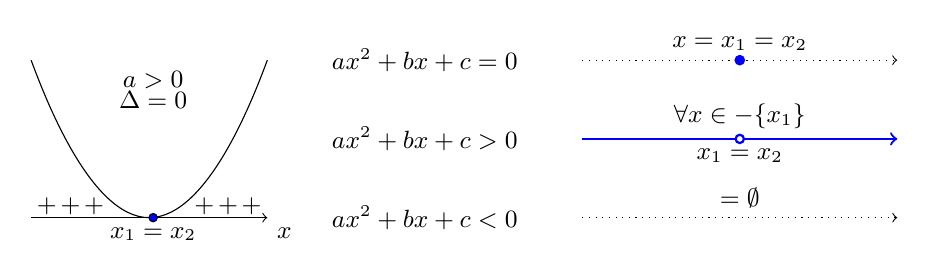
\begin{tikzpicture}[font=\small,x=10mm, y=10mm]

% seconda parabola;
  \draw (-1,0) parabola[parabola height=-2cm] +(3,0);
  \draw[->] (-1,-2) -- (2,-2) node [below right] () {$x$};
  \draw[fill=blue] (.55,-2)circle (1.5pt);
  \foreach \x in {-.8,-.5,-.2,1.2,1.5,1.8}{
  \node  at (\x,-1.85) {$+$};
  }
  \node[below] at (.55,-2) {$x_1=x_2$};
  \node[] at (.55,-.5) {$\Delta=0$};
  \node[] at (.55,-.25) {$a>0$};
%segno
  \node[] at (4,0) {$ax^2+bx+c=0$};
  \node[] at (4,-1) {$ax^2+bx+c>0$};
  \node[] at (4,-2) {$ax^2+bx+c<0$};
%Insieme soluzione

%primo insieme
\begin{scope}[dotted]
\draw (6,0) -- (8,0);
\draw[->] (8,0) -- (10,0);
\end{scope}
\node[above]  at (8,0) {$x=x_1=x_2$};
\begin{scope}[blue,thick]
\draw[fill=blue] (8,0)circle (1.5pt);
\end{scope}

%secondo insieme
\node[below]  at (8,-1) {$x_1=x_2$};
\node[above]  at (8,-1) {$\forall{x} \in \insR-\{x_1\}$};
\begin{scope}[blue,thick]
\draw[->] (6,-1) -- (10,-1);
\draw[fill=white] (8,-1)circle (1.5pt);
\end{scope}

%terzo insieme
\begin{scope}[dotted]
\draw[->] (6,-2) -- (10,-2);
\end{scope}
\node[above]  at (8,-2) {$\IS=\emptyset$};

\end{tikzpicture}

}
% \vspace{12pt}
% {% (c) 2013 Claudio Carboncini - claudio.carboncini@gmail.com
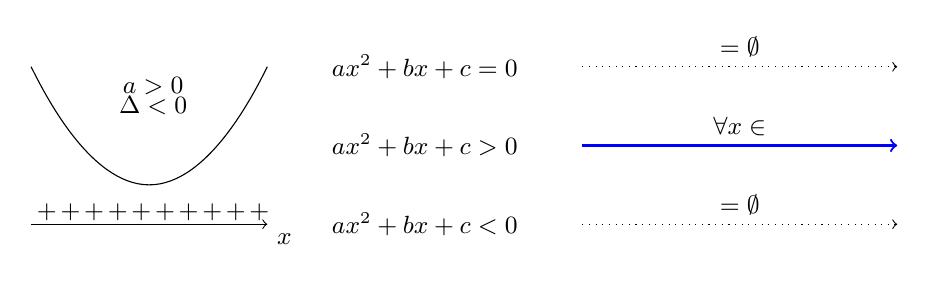
\begin{tikzpicture}[font=\small,x=10mm, y=10mm]

% terza parabola;
  \draw (-1,0) parabola[parabola height=-1.5cm] +(3,0);
  \draw[->] (-1,-2) -- (2,-2) node [below right] () {$x$};
  \foreach \x in {-.8,-.5,-.2,.1,.4,.7,1,1.3,1.6,1.9}{
  \node  at (\x,-1.85) {$+$};
  }
  \node[] at (.55,-.5) {$\Delta<0$};
  \node[] at (.55,-.25) {$a>0$};
%segno
  \node[] at (4,0) {$ax^2+bx+c=0$};
  \node[] at (4,-1) {$ax^2+bx+c>0$};
  \node[] at (4,-2) {$ax^2+bx+c<0$};
%Insieme soluzione
%primo insieme
\begin{scope}[dotted]
\draw[->] (6,0) -- (10,0);
\end{scope}
\node[above]  at (8,0) {$\IS=\emptyset$};
%secondo insieme
\node[above]  at (8,-1) {$\forall x \in \insR$};
\begin{scope}[blue,thick]
\draw[->] (6,-1) -- (10,-1);
\end{scope}
%terzo insieme
\begin{scope}[dotted]
\draw[->] (6,-2) -- (10,-2);
\end{scope}
\node[above]  at (8,-2) {$\IS=\emptyset$};

\end{tikzpicture}

}
% \vspace{12pt}
% {% (c) 2013 Claudio Carboncini - claudio.carboncini@gmail.com
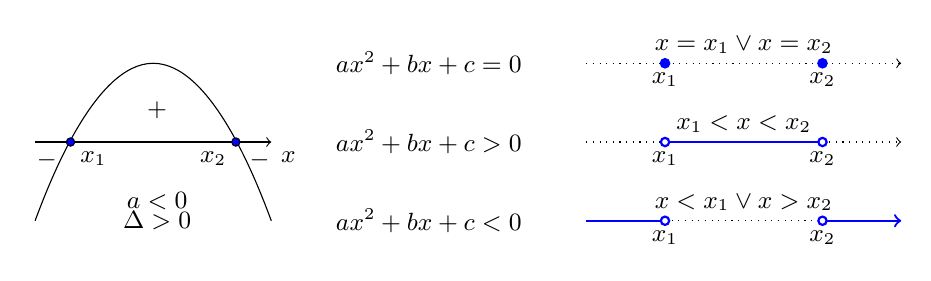
\begin{tikzpicture}[font=\small,x=10mm, y=10mm]

% prima parabola;
  \draw (-1,0) parabola[parabola height=2cm] +(3,0);
  \draw[->] (-1,1) -- (2,1) node [below right] () {$x$};
  \draw[fill=blue] (-.55,1)circle (1.5pt);
  \draw[fill=blue] (1.55,1)circle (1.5pt);
  \node[below right] at (-.55,1) {$x_1$};
  \node[below left] at (1.55,1) {$x_2$};
  \node[below right] at (1.6,1) {$-$};
  \node[below left] at (-.6,1) {$-$};
  \node[] at (.55,1.4) {$+$};
  \node[] at (.55,0) {$\Delta>0$};
  \node[] at (.55,.25) {$a<0$};
%segno
  \node[] at (4,2) {$ax^2+bx+c=0$};
  \node[] at (4,1) {$ax^2+bx+c>0$};
  \node[] at (4,0) {$ax^2+bx+c<0$};

%Insieme soluzione
%primo insieme
\begin{scope}[dotted]
\draw[->] (6,2) -- (10,2);
\end{scope}
\node[below]  at (7,2) {$x_1$};
\node[below]  at (9,2) {$x_2$};
\node[above]  at (8,2) {$x=x_1 \vee x=x_2$};
\begin{scope}[blue,thick]
\draw[fill=blue] (7,2)circle (1.5pt);
\draw[fill=blue] (9,2)circle (1.5pt);
\end{scope}
%secondo insieme
\begin{scope}[dotted]
\draw (6,1) -- (7,1);
\draw[->] (9,1) -- (10,1);
\end{scope}
\node[below]  at (7,1) {$x_1$};
\node[below]  at (9,1) {$x_2$};
\node[above]  at (8,1) {$x_1<x<x_2$};
\begin{scope}[blue,thick]
\draw (7,1) -- (9,1);
\draw[fill=white] (7,1)circle (1.5pt);
\draw[fill=white] (9,1)circle (1.5pt);
\end{scope}

%terzo insieme
\begin{scope}[dotted]
\draw (7,0) -- (9,0);
\end{scope}
\node[below]  at (7,0) {$x_1$};
\node[below]  at (9,0) {$x_2$};
\begin{scope}[blue,thick]
\draw (6,0) -- (7,0);
\draw[->] (9,0) -- (10,0);
\draw[fill=white] (7,0)circle (1.5pt);
\draw[fill=white] (9,0)circle (1.5pt);
\end{scope}
\node[above]  at (8,0) {$x<x_1 \vee x>x_2$};

\end{tikzpicture}

}
% \vspace{12pt}
% {% (c) 2013 Claudio Carboncini - claudio.carboncini@gmail.com
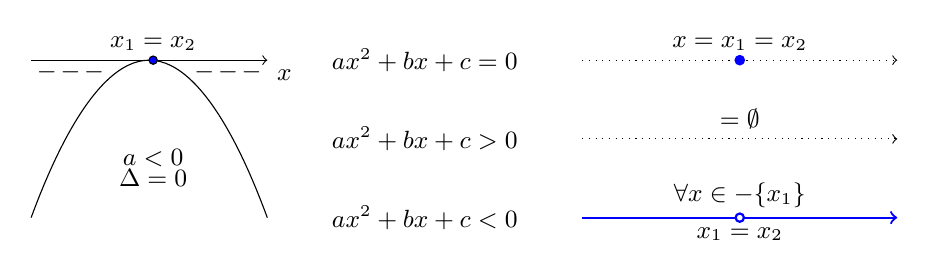
\begin{tikzpicture}[font=\small,x=10mm, y=10mm]

% quarta parabola;
  \draw (-1,0) parabola[parabola height=2cm] +(3,0);
  \draw[->] (-1,2) -- (2,2) node [below right] () {$x$};
  \draw[fill=blue] (.55,2)circle (1.5pt);
  \foreach \x in {-.8,-.5,-.2,1.2,1.5,1.8}{
  \node  at (\x,1.85) {$-$};
  }
  \node[above] at (.55,2) {$x_1=x_2$};
  \node[] at (.55,.5) {$\Delta=0$};
  \node[] at (.55,.75) {$a<0$};
%segno
  \node[] at (4,2) {$ax^2+bx+c=0$};
  \node[] at (4,1) {$ax^2+bx+c>0$};
  \node[] at (4,0) {$ax^2+bx+c<0$};
%Insieme soluzione

%primo insieme
\begin{scope}[dotted]
\draw (6,2) -- (8,2);
\draw[->] (8,2) -- (10,2);
\end{scope}
\node[above]  at (8,2) {$x=x_1=x_2$};
\begin{scope}[blue,thick]
\draw[fill=blue] (8,2)circle (1.5pt);
\end{scope}

%secondo insieme
\begin{scope}[dotted]
\draw[->] (6,1) -- (10,1);
\end{scope}
\node[above]  at (8,1) {$\IS=\emptyset$};

%terzo insieme
\node[below]  at (8,0) {$x_1=x_2$};
\node[above]  at (8,0) {$\forall x \in \insR-\{x_1\}$};
\begin{scope}[blue,thick]
\draw[->] (6,0) -- (10,0);
\draw[fill=white] (8,0)circle (1.5pt);
\end{scope}

\end{tikzpicture}

}
% \vspace{12pt}
% {% (c) 2013 Claudio Carboncini - claudio.carboncini@gmail.com
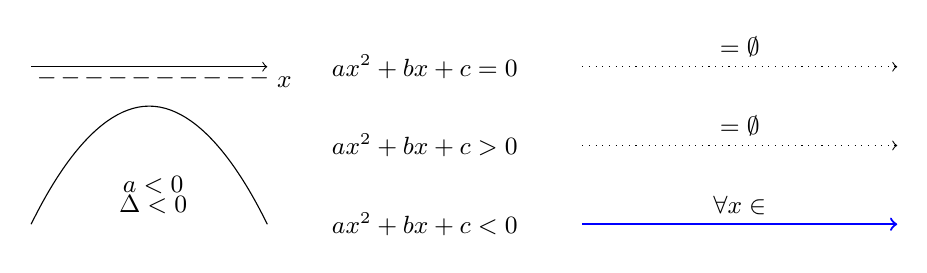
\begin{tikzpicture}[font=\small,x=10mm, y=10mm]

% ultima parabola;
  \draw (-1,0) parabola[parabola height=1.5cm] +(3,0);
  \draw[->] (-1,2) -- (2,2) node [below right] () {$x$};
  \foreach \x in {-.8,-.5,-.2,.1,.4,.7,1,1.3,1.6,1.9}{
    \node  at (\x,1.85) {$-$};
  }
  \node[] at (.55,.25) {$\Delta<0$};
  \node[] at (.55,.5) {$a<0$};
%segno
  \node[] at (4,2) {$ax^2+bx+c=0$};
  \node[] at (4,1) {$ax^2+bx+c>0$};
  \node[] at (4,0) {$ax^2+bx+c<0$};
%Insieme soluzione
%primo insieme
\draw[->, dotted] (6,2) -- (10,2);
\node[above]  at (8,2) {$\IS=\emptyset$};
%secondo insieme
\draw[->, dotted] (6, 1) -- (10, 1);
\node[above]  at (8, 1) {$\IS=\emptyset$};
%terzo insieme
\draw[->, blue,thick] (6, 0) -- (10, 0);
\node[above]  at (8, 0) {$\forall x \in \insR$};

\end{tikzpicture}

}
% \caption{Risoluzione delle disequazioni di secondo grado}
% \label{fig:subfig10}
% \end{figure}
% \end{inaccessibleblock}

\begin{inaccessibleblock}[I sei casi di posizione di una parabola rispetto 
  all'asse~x.]
\end{inaccessibleblock}

{\centering
% (c) 2013 Claudio Carboncini - claudio.carboncini@gmail.com
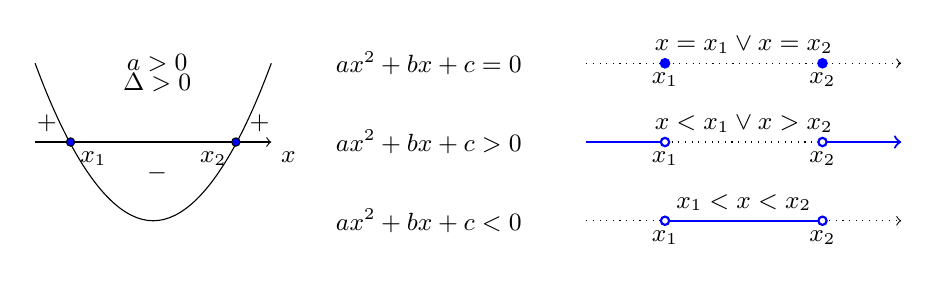
\begin{tikzpicture}[font=\small,x=10mm, y=10mm]

% prima parabola;
  \draw (-1,0) parabola[parabola height=-2cm] +(3,0);
  \draw[->] (-1,-1) -- (2,-1) node [below right] () {$x$};
  \draw[fill=blue] (-.55,-1)circle (1.5pt);
  \draw[fill=blue] (1.55,-1)circle (1.5pt);
  \node[below right] at (-.55,-1) {$x_1$};
  \node[below left] at (1.55,-1) {$x_2$};
  \node[above right] at (1.6,-1) {$+$};
  \node[above left] at (-.6,-1) {$+$};
  \node[] at (.55,-1.4) {$-$};
  \node[] at (.55,-.25) {$\Delta>0$};
  \node[] at (.55,0) {$a>0$};
%segno
  \node[] at (4,0) {$ax^2+bx+c=0$};
  \node[] at (4,-1) {$ax^2+bx+c>0$};
  \node[] at (4,-2) {$ax^2+bx+c<0$};

%Insieme soluzione
%primo insieme
\begin{scope}[dotted]
\draw[->] (6,0) -- (10,0);
\end{scope}
\node[below]  at (7,0) {$x_1$};
\node[below]  at (9,0) {$x_2$};
\node[above]  at (8,0) {$x=x_1 \vee x=x_2$};
\begin{scope}[blue,thick]
\draw[fill=blue] (7,0)circle (1.5pt);
\draw[fill=blue] (9,0)circle (1.5pt);
\end{scope}
%secondo insieme
\begin{scope}[dotted]
\draw (7,-1) -- (9,-1);
\end{scope}
\node[below]  at (7,-1) {$x_1$};
\node[below]  at (9,-1) {$x_2$};
\node[above]  at (8,-1) {$x<x_1 \vee x>x_2$};
\begin{scope}[blue,thick]
\draw (6,-1) -- (7,-1);
\draw[->] (9,-1) -- (10,-1);
\draw[fill=white] (7,-1)circle (1.5pt);
\draw[fill=white] (9,-1)circle (1.5pt);
\end{scope}

%terzo insieme
\begin{scope}[dotted]
\draw (6,-2) -- (7,-2);
\draw[->] (9,-2) -- (10,-2);
\end{scope}
\node[below]  at (7,-2) {$x_1$};
\node[below]  at (9,-2) {$x_2$};
\begin{scope}[blue,thick]
\draw (7,-2) -- (9,-2);
\draw[fill=white] (7,-2)circle (1.5pt);
\draw[fill=white] (9,-2)circle (1.5pt);
\end{scope}
\node[above]  at (8,-2) {$x_1<x<x_2$};

\end{tikzpicture}


\vspace{12pt}
% (c) 2013 Claudio Carboncini - claudio.carboncini@gmail.com
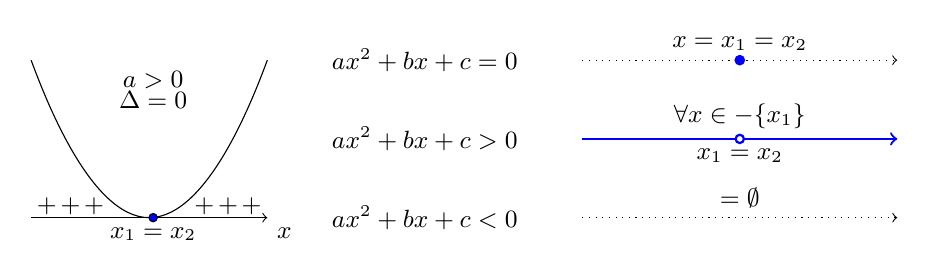
\begin{tikzpicture}[font=\small,x=10mm, y=10mm]

% seconda parabola;
  \draw (-1,0) parabola[parabola height=-2cm] +(3,0);
  \draw[->] (-1,-2) -- (2,-2) node [below right] () {$x$};
  \draw[fill=blue] (.55,-2)circle (1.5pt);
  \foreach \x in {-.8,-.5,-.2,1.2,1.5,1.8}{
  \node  at (\x,-1.85) {$+$};
  }
  \node[below] at (.55,-2) {$x_1=x_2$};
  \node[] at (.55,-.5) {$\Delta=0$};
  \node[] at (.55,-.25) {$a>0$};
%segno
  \node[] at (4,0) {$ax^2+bx+c=0$};
  \node[] at (4,-1) {$ax^2+bx+c>0$};
  \node[] at (4,-2) {$ax^2+bx+c<0$};
%Insieme soluzione

%primo insieme
\begin{scope}[dotted]
\draw (6,0) -- (8,0);
\draw[->] (8,0) -- (10,0);
\end{scope}
\node[above]  at (8,0) {$x=x_1=x_2$};
\begin{scope}[blue,thick]
\draw[fill=blue] (8,0)circle (1.5pt);
\end{scope}

%secondo insieme
\node[below]  at (8,-1) {$x_1=x_2$};
\node[above]  at (8,-1) {$\forall{x} \in \insR-\{x_1\}$};
\begin{scope}[blue,thick]
\draw[->] (6,-1) -- (10,-1);
\draw[fill=white] (8,-1)circle (1.5pt);
\end{scope}

%terzo insieme
\begin{scope}[dotted]
\draw[->] (6,-2) -- (10,-2);
\end{scope}
\node[above]  at (8,-2) {$\IS=\emptyset$};

\end{tikzpicture}


\vspace{12pt}
% (c) 2013 Claudio Carboncini - claudio.carboncini@gmail.com
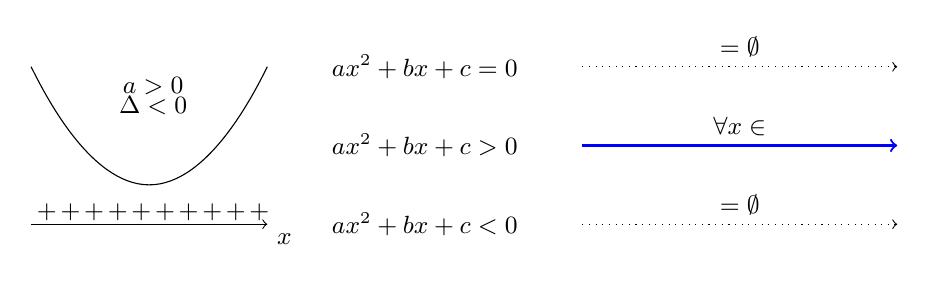
\begin{tikzpicture}[font=\small,x=10mm, y=10mm]

% terza parabola;
  \draw (-1,0) parabola[parabola height=-1.5cm] +(3,0);
  \draw[->] (-1,-2) -- (2,-2) node [below right] () {$x$};
  \foreach \x in {-.8,-.5,-.2,.1,.4,.7,1,1.3,1.6,1.9}{
  \node  at (\x,-1.85) {$+$};
  }
  \node[] at (.55,-.5) {$\Delta<0$};
  \node[] at (.55,-.25) {$a>0$};
%segno
  \node[] at (4,0) {$ax^2+bx+c=0$};
  \node[] at (4,-1) {$ax^2+bx+c>0$};
  \node[] at (4,-2) {$ax^2+bx+c<0$};
%Insieme soluzione
%primo insieme
\begin{scope}[dotted]
\draw[->] (6,0) -- (10,0);
\end{scope}
\node[above]  at (8,0) {$\IS=\emptyset$};
%secondo insieme
\node[above]  at (8,-1) {$\forall x \in \insR$};
\begin{scope}[blue,thick]
\draw[->] (6,-1) -- (10,-1);
\end{scope}
%terzo insieme
\begin{scope}[dotted]
\draw[->] (6,-2) -- (10,-2);
\end{scope}
\node[above]  at (8,-2) {$\IS=\emptyset$};

\end{tikzpicture}


\vspace{12pt}
% (c) 2013 Claudio Carboncini - claudio.carboncini@gmail.com
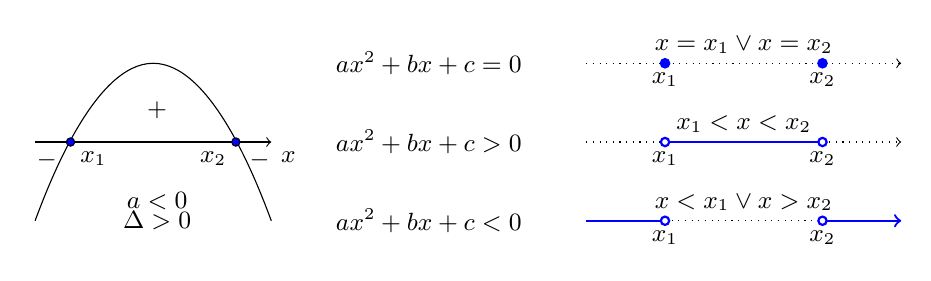
\begin{tikzpicture}[font=\small,x=10mm, y=10mm]

% prima parabola;
  \draw (-1,0) parabola[parabola height=2cm] +(3,0);
  \draw[->] (-1,1) -- (2,1) node [below right] () {$x$};
  \draw[fill=blue] (-.55,1)circle (1.5pt);
  \draw[fill=blue] (1.55,1)circle (1.5pt);
  \node[below right] at (-.55,1) {$x_1$};
  \node[below left] at (1.55,1) {$x_2$};
  \node[below right] at (1.6,1) {$-$};
  \node[below left] at (-.6,1) {$-$};
  \node[] at (.55,1.4) {$+$};
  \node[] at (.55,0) {$\Delta>0$};
  \node[] at (.55,.25) {$a<0$};
%segno
  \node[] at (4,2) {$ax^2+bx+c=0$};
  \node[] at (4,1) {$ax^2+bx+c>0$};
  \node[] at (4,0) {$ax^2+bx+c<0$};

%Insieme soluzione
%primo insieme
\begin{scope}[dotted]
\draw[->] (6,2) -- (10,2);
\end{scope}
\node[below]  at (7,2) {$x_1$};
\node[below]  at (9,2) {$x_2$};
\node[above]  at (8,2) {$x=x_1 \vee x=x_2$};
\begin{scope}[blue,thick]
\draw[fill=blue] (7,2)circle (1.5pt);
\draw[fill=blue] (9,2)circle (1.5pt);
\end{scope}
%secondo insieme
\begin{scope}[dotted]
\draw (6,1) -- (7,1);
\draw[->] (9,1) -- (10,1);
\end{scope}
\node[below]  at (7,1) {$x_1$};
\node[below]  at (9,1) {$x_2$};
\node[above]  at (8,1) {$x_1<x<x_2$};
\begin{scope}[blue,thick]
\draw (7,1) -- (9,1);
\draw[fill=white] (7,1)circle (1.5pt);
\draw[fill=white] (9,1)circle (1.5pt);
\end{scope}

%terzo insieme
\begin{scope}[dotted]
\draw (7,0) -- (9,0);
\end{scope}
\node[below]  at (7,0) {$x_1$};
\node[below]  at (9,0) {$x_2$};
\begin{scope}[blue,thick]
\draw (6,0) -- (7,0);
\draw[->] (9,0) -- (10,0);
\draw[fill=white] (7,0)circle (1.5pt);
\draw[fill=white] (9,0)circle (1.5pt);
\end{scope}
\node[above]  at (8,0) {$x<x_1 \vee x>x_2$};

\end{tikzpicture}


\vspace{12pt}
% (c) 2013 Claudio Carboncini - claudio.carboncini@gmail.com
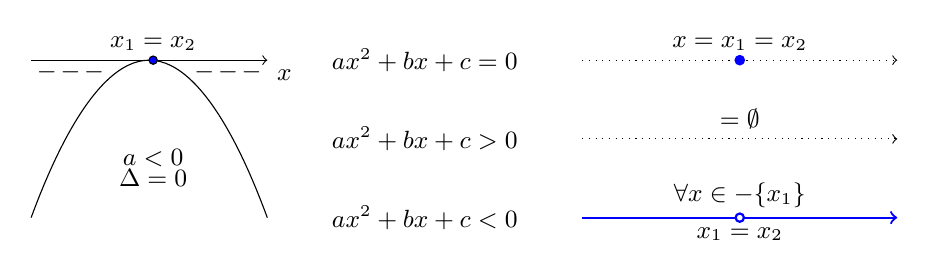
\begin{tikzpicture}[font=\small,x=10mm, y=10mm]

% quarta parabola;
  \draw (-1,0) parabola[parabola height=2cm] +(3,0);
  \draw[->] (-1,2) -- (2,2) node [below right] () {$x$};
  \draw[fill=blue] (.55,2)circle (1.5pt);
  \foreach \x in {-.8,-.5,-.2,1.2,1.5,1.8}{
  \node  at (\x,1.85) {$-$};
  }
  \node[above] at (.55,2) {$x_1=x_2$};
  \node[] at (.55,.5) {$\Delta=0$};
  \node[] at (.55,.75) {$a<0$};
%segno
  \node[] at (4,2) {$ax^2+bx+c=0$};
  \node[] at (4,1) {$ax^2+bx+c>0$};
  \node[] at (4,0) {$ax^2+bx+c<0$};
%Insieme soluzione

%primo insieme
\begin{scope}[dotted]
\draw (6,2) -- (8,2);
\draw[->] (8,2) -- (10,2);
\end{scope}
\node[above]  at (8,2) {$x=x_1=x_2$};
\begin{scope}[blue,thick]
\draw[fill=blue] (8,2)circle (1.5pt);
\end{scope}

%secondo insieme
\begin{scope}[dotted]
\draw[->] (6,1) -- (10,1);
\end{scope}
\node[above]  at (8,1) {$\IS=\emptyset$};

%terzo insieme
\node[below]  at (8,0) {$x_1=x_2$};
\node[above]  at (8,0) {$\forall x \in \insR-\{x_1\}$};
\begin{scope}[blue,thick]
\draw[->] (6,0) -- (10,0);
\draw[fill=white] (8,0)circle (1.5pt);
\end{scope}

\end{tikzpicture}


\vspace{12pt}
% (c) 2013 Claudio Carboncini - claudio.carboncini@gmail.com
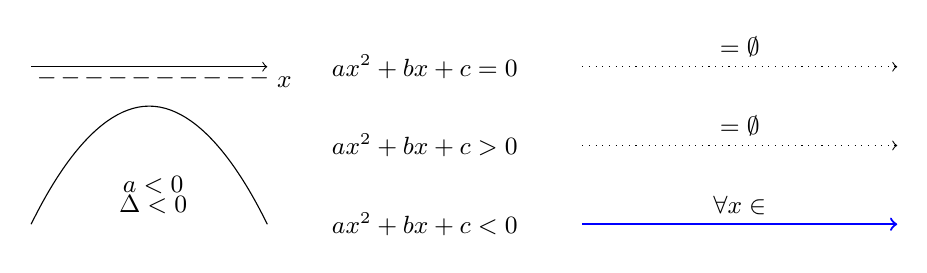
\begin{tikzpicture}[font=\small,x=10mm, y=10mm]

% ultima parabola;
  \draw (-1,0) parabola[parabola height=1.5cm] +(3,0);
  \draw[->] (-1,2) -- (2,2) node [below right] () {$x$};
  \foreach \x in {-.8,-.5,-.2,.1,.4,.7,1,1.3,1.6,1.9}{
    \node  at (\x,1.85) {$-$};
  }
  \node[] at (.55,.25) {$\Delta<0$};
  \node[] at (.55,.5) {$a<0$};
%segno
  \node[] at (4,2) {$ax^2+bx+c=0$};
  \node[] at (4,1) {$ax^2+bx+c>0$};
  \node[] at (4,0) {$ax^2+bx+c<0$};
%Insieme soluzione
%primo insieme
\draw[->, dotted] (6,2) -- (10,2);
\node[above]  at (8,2) {$\IS=\emptyset$};
%secondo insieme
\draw[->, dotted] (6, 1) -- (10, 1);
\node[above]  at (8, 1) {$\IS=\emptyset$};
%terzo insieme
\draw[->, blue,thick] (6, 0) -- (10, 0);
\node[above]  at (8, 0) {$\forall x \in \insR$};

\end{tikzpicture}


}

% %%%%%%%%%%%%%%%%%%%%%%%%%%%%%
% \osservazione Per semplificare le varie tipologie di configurazione si può 
% supporre ch eil coefficiente di $x^2$, cioè il coefficiente a, sia positivo. 
% Se 
% così non fosse basterebbe moltiplicare per (-1)entrambi i membri della 
% disequazione e cambiare segno a tutti gli addendi. Nell'esempio appena svolto 
% da 
% $-3x^2+2x>0$ si otterrebbe $3x^2-2x<0$. La risoluzione di questa 
% disequazione, 
% ottenuta dopo il cambio del segno, chiede che si cerchino i valori delle 
% ascisse 
% x dei punti del grafico che hanno le ordinate y negative, cioè  $y<0$ , 
% essendo 
% $y=3x^2-2x$ l'equazione della parabola associata.La parabola associata ha le 
% stesse intersezioni con l'asse delle x di quella dell'esempio, ma non la 
% concavità che in questo caso è rivolta verso l'alto , infatti $a=3>0$.Riporta 
% qui a lato la configrazione della parabola.
% Da essa puoi osservare che i punti del grafico con ordinata negativa sono 
% quelli 
% la cui ascissa è compresa fra le ascisse dei due punti di intersezione con 
% l'asse delle x.
% L'insieme delle soluzioni è pertanto $\IS=\left\{x\in \insR | 0<x<\frac 2 
% 3\right\}$, come sopra nell'esempio.
% 
% %%%%%%%%%%%%%%%%%%%%%%%%%%%%%%
% \section{Segno del trinomio a coefficienti letterali}
% Consideriamo il trinomio $t=kx^2+3x-7$ di secondo grado avente il primo 
% coefficiente dipendente dal parametro $k$. Come possiamo stabilire il segno 
% di 
% questo trinomio, al variare di $k$?
% Sappiamo che stabilire il segno di un trinomio significa determinare i valori 
% reali che attribuiti alla variabile indipendente $x$ rendono il trinomio 
% positivo, nullo o negativo. Evidentemente per valori reali diversi di $k$ 
% avremo 
% una diversa disequazione da risolvere; dobbiamo dunque cercare di analizzare 
% come varia il trinomio a seconda dei valori di $k$ e in seguito studiare il 
% segno del trinomio ottenuto. Questa analisi di situazioni diverse è la 
% \textit{discussione del trinomio a coefficienti parametrici}.
% 
% %%%%%%%%%%%%%%%%%%%%%%%%%%%%%%
% \conclusione Una disequazione di secondo grado si presenta sempre in una 
% delle 
% seguenti forme: ${ax}^2+{bx}+c>0$, ${ax}^2+{bx}+c\ge 0$, ${ax}^2+{bx}+c<0$, 
% ${ax}^2+{bx}+c\le 0$ possiamo sempre supporre positivo il primo coefficiente 
% e, 
% anche se incompleta, per l'equazione associata possiamo sempre pensare ai tre 
% casi generati dal segno del discriminante $\Delta =b^2-4{ac}$. Pertanto 
% avremo:
% 
% %%%%%%%%%%%%%%%%%%%%%%%%%%%%%
% % \begin{exrig}
% \begin{esempio}
% Stabilire il segno di $t=kx^2+3x-7$ al variare di $ k $.
% 
% Prendiamo in considerazione il segno del primo coefficiente e il segno del 
% discriminante dell'equazione associata $kx^2+3x-7=0$. Il primo coefficiente è 
% maggiore di zero per $k>0$. Il discriminante $\Delta =9+28k$ è maggiore di 
% zero 
% per $k>-\frac 9{28}$. Rappresentiamo la loro reciproca situazione:
% \begin{center}
% %%%%%%%%%%%%%%%%%%%%%%%%%%%%%%
% \begin{threeparttable}
% \begin{tabular}{lllll}
% \toprule
% Delta & $ax^2+bx+c>0$& $ax^2+bx+c\ge0$& $ax^2+bx+c<0$ & $ax^2+bx+c\le0$\\
% \midrule
%  $\Delta >0^{*}$& $ x<x_1\vee x>x_2 $ & $ x\le x_1\vee x\ge x_2 $& $ 
% x_1<x<x_2 
% $&$ x_1\le x\le x_2 $\\
% $\Delta =0^{**}$& $\forall x\in \insR-\{x_1\} $ & $ \forall x\in \insR $& $ 
% \IS=\emptyset $&$ x=x_1=x_2 $\\
% $\Delta <0^{***}$&$ \forall x\in \insR $ & $ \forall x\in \insR $& $ 
% \IS=\emptyset $&$ \IS=\emptyset $\\
% \bottomrule
% \end{tabular}
% \begin{tablenotes}
% \item [*] L'equazione associata ha 2 soluzioni reali distinte: $x=x_1\vee 
% x=x_2$.
% \item [**] L'equazione associata ha 2 soluzioni reali coincidenti: 
% $x=x_1=x_2$.
% \item [***] L'equazione associata non ha soluzioni reali.
% \end{tablenotes}
% \end{threeparttable}
% \end{center}
% %%%%%%%%%%%%%%%%%%%%%%%%%%%%%%
%  % (c) 2013 Claudio Carboncini - claudio.carboncini@gmail.com
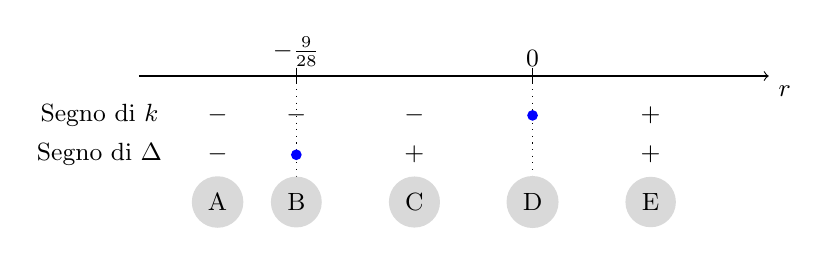
\begin{tikzpicture}[font=\small,x=10mm, y=10mm]

\draw[->] (0,0) -- (8,0) node [below right] () {$r$};

\foreach \x in {2,5}{
\draw(\x,3pt)--(\x,-3pt);
\begin{scope}[dotted]
\draw (\x,0) -- (\x,-1.5);
\end{scope}}
\node[] at (-.5,-0.5) {Segno di $k$};
\node[] at (-.5,-1) {Segno di $\Delta$};
\node[above]  at (2,0) {$-\frac{9}{28}$};
\node[above]  at (5,0) {$0$};
\node[] at (1,-0.5) {$-$};
\node[] at (2,-0.5) {$-$};
\node[] at (3.5,-0.5) {$-$};
\node[] at (6.5,-0.5) {$+$};
\node[] at (1,-1) {$-$};
\node[] at (3.5,-1) {$+$};
\node[] at (6.5,-1) {$+$};
\node [circle,fill=gray!30](A) at (1,-1.6) {A};
\node [circle,fill=gray!30](B) at (2,-1.6) {B};
\node [circle,fill=gray!30](C) at (3.5,-1.6) {C};
\node [circle,fill=gray!30](D) at (5,-1.6) {D};
\node [circle,fill=gray!30](E) at (6.5,-1.6) {E};

\begin{scope}[blue,thick]
\draw[fill=blue] (5,-.5)circle (1.5pt);
\draw[fill=blue] (2,-1)circle (1.5pt);
\end{scope}

\end{tikzpicture}

% % \end{center}
% \vspazio\ovalbox{\risolvii \ref{ese:4.1}, \ref{ese:4.2}, \ref{ese:4.3}, 
% \ref{ese:4.4}, \ref{ese:4.5}, \ref{ese:4.6}}
% 
% \end{esempio}
% 
% %%%%%%%%%%%%%%%%%%%%%%%%%%%%%%
% % \end{exrig}


\section{Disequazioni polinomiali di grado superiore}
\label{sec:diseq_grado_superiore}

\begin{procedura}
Risolvere le disequazioni di grado superiore:
\begin{enumeratea}
\item scomponi il polinomio di grado $n$ in fattori di primo e secondo grado;
\item studia il segno dei singoli fattori;
\item costruisci la tabella dei segni;
\item cerca gli intervalli in cui il polinomio dato assume il segno richiesto.
\item rappresenta, con i diversi metodi visti, gli intervalli che 
 risolvono la disequazione.
\end{enumeratea}
\end{procedura}

Applichiamo la procedura ai seguenti esempi.

% \begin{exrig}
\begin{esempio}
 \[p(x)=-2x^3+3x^2+8x-12 \le 0\]

In questo caso dobbiamo risolvere una disequazione di terzo grado. 
Possiamo ridurre la difficoltà scomponendo in fattori il polinomio in modo da 
ottenere il prodotto di più polinomi di primo grado: 

\begin{align*}
P(x) = -2x^3+3x^2+8x-12 &= x^2(-2x+3)-4(-2x+3) = \\
                        &= (x^2-4)(-2x+3) = \\
                        &= (x-2)(x+2)(-2x+3) \le 0
\end{align*}

\begin{minipage}{.65\textwidth}

A questo punto possiamo studiare il segno dei polinomi, applicando la regola 
dei segni di un prodotto trovare il segno del polinomio e risolvere la 
disequazione.

\end{minipage}
\begin{minipage}{.30\textwidth}

\begin{inaccessibleblock}[Regola dei segni nella moltiplicazione]
\begin{center}
  % (c) 2012 Dimitrios Vrettos - d.vrettos@gmail.com
\begin{tikzpicture}[font=\small,x=10mm, y=10mm]

\matrix (a)[matrix of nodes]{
$\times$& $+$ $-$\\
$+$& $+$ $-$\\
$-$& $-$ $+$\\
};

\begin{scope}[orange]
\draw (a-1-1.north east)--(a-3-1.south east);
\draw (a-1-1.south west)--(a-1-2.south east);
\end{scope}
\end{tikzpicture}
\end{center}
\end{inaccessibleblock}
\end{minipage}

\newpage %----------------------------------------------

Studiamo il segno di ogni singolo fattore:
\begin{itemize}
 \item segno di $(x-2)$\\
 \begin{minipage}{.45\textwidth}
  E.A.:~$x-2=0 \Rightarrow x=2$
 \end{minipage}
 \begin{minipage}{.25\textwidth}
  F.A.:~$y=x-2 \rightarrow $
 \end{minipage}
 \begin{minipage}{.3\textwidth}
  \begin{inaccessibleblock}[retta crescente con zero in~2]
  % (c) 2014 Daniele Zambelli - daniele.zambelli@gmail.com

%%%
% Retta crescente zero in 2
%%%%
 
\begin{tikzpicture}[x=1.5mm, y=1.5mm, smooth]

% (c) 2014 Daniele Zambelli - daniele.zambelli@gmail.com

%%%
% Retta crescente con segni
%%%%
 
\coordinate (inizio) at (-10, -4);
\coordinate (zero) at (0, 0);
\coordinate (fine) at (10, 4);

% (c) 2014 Daniele Zambelli - daniele.zambelli@gmail.com

%%%
% Asse cartesiano x
%%%%

\input{lbr/assiepiani/asse10.pgf}
\node [below] at (10, 0)  {$x$};


\draw [-] [ultra thick, red!50!black] (inizio) -- (zero);
\draw [-] [ultra thick, blue!50!black] (zero) -- (fine);

\node [xshift=-25, yshift=-3, above] at (zero) {$-$};
\draw[blue, thick, fill=white] (zero) circle (2pt);
\node [xshift=25, yshift=-3, above] at (zero) {$+$};

\node [above] {$+2$};

\end{tikzpicture}

\end{inaccessibleblock}
 \end{minipage}
 \item segno di $(x+2)$\\
 \begin{minipage}{.45\textwidth}
  E.A.:~$x+2=0 \Rightarrow x=\frac{1}{2}$
 \end{minipage}
 \begin{minipage}{.25\textwidth}
  F.A.:~$y=x+2 \rightarrow $
 \end{minipage}
 \begin{minipage}{.3\textwidth}
  \begin{inaccessibleblock}[retta crescente con zero in~-2]
  % (c) 2014 Daniele Zambelli - daniele.zambelli@gmail.com

%%%
% Retta decrescente zero in 1/2
%%%%
 
\begin{tikzpicture}[x=1.5mm, y=1.5mm, smooth]

% (c) 2014 Daniele Zambelli - daniele.zambelli@gmail.com

%%%
% Retta decrescente con segni
%%%%
 
\coordinate (inizio) at (-10, 4);
\coordinate (zero) at (0, 0);
\coordinate (fine) at (10, -4);

% (c) 2014 Daniele Zambelli - daniele.zambelli@gmail.com

%%%
% Asse cartesiano x
%%%%

\input{lbr/assiepiani/asse10.pgf}
\node [below] at (10, 0)  {$x$};


\draw [-] [ultra thick, blue!50!black] (inizio) -- (zero);
\draw [-] [ultra thick, red!50!black] (zero) -- (fine);

\node [xshift=-25, yshift=-3, above] at (zero) {$+$};
\draw[blue, thick, fill=white] (zero) circle (2pt);
\node [xshift=25, yshift=-3, above] at (zero) {$-$};

\node [above] {$\frac{1}{2}$};

\end{tikzpicture}

\end{inaccessibleblock}
 \end{minipage}
 \item Segno del denominatore:\\
 \begin{minipage}{.45\textwidth}
  E.A.:~$-2x+3=0 \Rightarrow x=\frac{3}{2}$
 \end{minipage}
 \begin{minipage}{.25\textwidth}
  F.A.:~$y=-2x+3 \rightarrow $
 \end{minipage}
 \begin{minipage}{.3\textwidth}
  \begin{inaccessibleblock}[retta decrescente con zero in~3/2]
  % (c) 2014 Daniele Zambelli - daniele.zambelli@gmail.com

%%%
% Retta decrescente zero in 1/2
%%%%
 
\begin{tikzpicture}[x=1.5mm, y=1.5mm, smooth]

% (c) 2014 Daniele Zambelli - daniele.zambelli@gmail.com

%%%
% Retta decrescente con segni
%%%%
 
\coordinate (inizio) at (-10, 4);
\coordinate (zero) at (0, 0);
\coordinate (fine) at (10, -4);

% (c) 2014 Daniele Zambelli - daniele.zambelli@gmail.com

%%%
% Asse cartesiano x
%%%%

\input{lbr/assiepiani/asse10.pgf}
\node [below] at (10, 0)  {$x$};


\draw [-] [ultra thick, blue!50!black] (inizio) -- (zero);
\draw [-] [ultra thick, red!50!black] (zero) -- (fine);

\node [xshift=-25, yshift=-3, above] at (zero) {$+$};
\draw[blue, thick, fill=white] (zero) circle (2pt);
\node [xshift=25, yshift=-3, above] at (zero) {$-$};

\node [above] {$\frac{3}{2}$};

\end{tikzpicture}

\end{inaccessibleblock}
 \end{minipage}
 \item Con la regola dei segni calcolo il segno della frazione 
\begin{inaccessibleblock}[Grafo con i segni]
  % (c) 2014 Daniele Zambelli - daniele.zambelli@gmail.com

%%%
% Studio dei segni di un prodotto
%%%%
 
\begin{tikzpicture}[x=2.5mm, y=5mm, smooth]

\coordinate (a_top) at (-5, 1);
\coordinate (a_bottom) at (-5, -3);
\coordinate (b_top) at (0, 1);
\coordinate (b_bottom) at (0, -3);
\coordinate (c_top) at (5, 1);
\coordinate (c_bottom) at (5, -3);

% (c) 2014 Daniele Zambelli - daniele.zambelli@gmail.com

%%%
% Grafo per il calcolo del segno con tre assi
%%%%
 
% (c) 2014 Daniele Zambelli - daniele.zambelli@gmail.com

%%%
% Asse cartesiano x
%%%%

\input{lbr/assiepiani/asse10.pgf}
\node [below] at (10, 0)  {$x$};

\begin{scope}[yshift= -.5cm]
  % (c) 2014 Daniele Zambelli - daniele.zambelli@gmail.com

%%%
% Asse cartesiano x
%%%%

\input{lbr/assiepiani/asse10.pgf}
\node [below] at (10, 0)  {$x$};

  \begin{scope}[yshift= -.5cm]
    % (c) 2014 Daniele Zambelli - daniele.zambelli@gmail.com

%%%
% Asse cartesiano x
%%%%

\input{lbr/assiepiani/asse10.pgf}
\node [below] at (10, 0)  {$x$};

    \begin{scope}[yshift= -.5cm]
      % (c) 2014 Daniele Zambelli - daniele.zambelli@gmail.com

%%%
% Asse cartesiano x
%%%%

\input{lbr/assiepiani/asse10.pgf}
\node [below] at (10, 0)  {$x$};

    \end{scope}
  \end{scope}
\end{scope}

\draw [-] [] (a_top) -- (a_bottom);
\draw [-] [] (b_top) -- (b_bottom);
\draw [-] [] (c_top) -- (c_bottom);

\node [above] at (-5, 1) {$-2$};
\node [above] at (0, 1) {$+\frac{3}{2}$};
\node [above] at (5, 1) {$+2$};

\node [above left] at (-10, 0) {$x-2$};
\node [above] at (-7.5, 0) {$-$};
\node [above] at (-2.5, 0) {$-$};
\node [above] at (2.5, 0) {$-$};
\draw (5, .5) circle (3pt);
\node [above] at (7.5, 0) {$+$};

\node [above left] at (-10, -1) {$x+2$};
\node [above] at (-7.5, -1) {$-$};
\draw (-5, -.5) circle (3pt);
\node [above] at (-2.5, -1) {$+$};
\node [above] at (2.5, -1) {$+$};
\node [above] at (7.5, -1) {$+$};

\node [above left] at (-10, -2) {$-2x+3$};
\node [above] at (-7.5, -2) {$+$};
% \draw (0 -.4, -1.5 -.2) -- (0 +.4, -1.5 +.2) 
%       (0 -.4, -1.5 +.2) -- (0 +.4, -1.5 -.2);
\node [above] at (-2.5, -2) {$+$};
\draw (0, -1.5) circle (3pt);
\node [above] at (2.5, -2) {$-$};
\node [above] at (7.5, -2) {$-$};

\node [above left] at (-10, -3.15) {$P(x)$};
\node [above] at (-7.5, -3) {$+$};
\draw (-5, -2.5) circle (3pt);
\node [above] at (-2.5, -3) {$-$};
\draw (0, -2.5) circle (3pt);
\node [above] at (2.5, -3) {$+$};
\draw (5, -2.5) circle (3pt);
\node [above] at (7.5, -3) {$-$};

\end{tikzpicture}
 
\end{inaccessibleblock}
 \item Quindi i valori di~$x$ che rendono vera la disequazione, cioè i valori
  che rendono~$f(x)$ non positivo, sono quelli 
  che si trovano a sinistra di~$-2$ oppure che si trovano a destra di~$+3$. 
 \subitem 
  \begin{minipage}{.35\textwidth}
   rappresentazione grafica: 
  \end{minipage}
  \begin{minipage}{.30\textwidth}
\begin{inaccessibleblock}[Retta con gli intervalli evidenziati]
   % (c) 2014 Daniele Zambelli - daniele.zambelli@gmail.com

%%%
% Valori esterni all'intervallo -2; 3
%%%%
 
\begin{tikzpicture}[x=1.5mm, y=1.5mm, smooth]

% \clip (-7.5, -5.5) rectangle (10.9, 10.9);

\coordinate (m_i) at (-10, 0);
\coordinate (a) at (-5, 0);
\coordinate (b) at (0, 0);
\coordinate (c) at (5, 0);
\coordinate (p_i) at (10, 0);

% (c) 2014 Daniele Zambelli - daniele.zambelli@gmail.com

%%%
% Asse cartesiano x
%%%%

% (c) 2014 Daniele Zambelli - daniele.zambelli@gmail.com

%%%
% Asse cartesiano generico
%%%%

\draw [-{Stealth[length=2mm, open, round]}] (-10, 0) -- (10, 0);

\node [below] at (10, 0)  {$x$};


\begin{scope}[blue,thick]
\draw [-,decorate,decoration=snake] (m_i) -- (a);
\draw[fill=white] (a) circle (2pt) node [above] {$-3$};
\draw [-,decorate,decoration=snake] (b) -- (c);
\draw[fill] (b) circle (2pt) node [above] {$\frac{1}{2}$};
\draw [fill=white] (c) -- (p_i);
\draw[fill] (c) circle (2pt) node [above] {$2$};
\end{scope}

\end{tikzpicture}

\end{inaccessibleblock}
  \end{minipage}
 \subitem rappresentazione con i 
   predicati:~$-2 \le x \le \frac{3}{2} \quad \lor \quad x \ge 2$ 
 \subitem rappresentazione con le 
  parentesi:~$]-2;~-3[ \quad \cup \quad [2;~+\infty]$. 
\end{itemize}

\end{esempio}

\begin{esempio}
Data la disequazione $-2x(3-2x)-3x^2\left(2-\frac 3 2x\right)\ge 
5\left(2x^2-\frac 3{10}x\right)$ determinate il suo $ \IS $

Osserviamo che la disequazione proposta è polinomiale di terzo grado; eseguiamo 
i calcoli per portarla alla forma $p(x)\ge 0$. Si ottiene $3x^3-8x^2-3x\ge 0$ e 
con la scomposizione \ si ha $x\cdot (3x^2-8x-3)\ge 0$. Procediamo con lo 
studio 
dei segni dei singoli fattori: $f_1\ge 0\rightarrow x\ge 0$ e $f_2\ge 
0\rightarrow x\le -\frac 1 3\vee x\ge 3$ e compiliamo \ la tabella dei segni 
che 
lasciamo al lettore.
\begin{center}
 % (c) 2013 Claudio Carboncini - claudio.carboncini@gmail.com
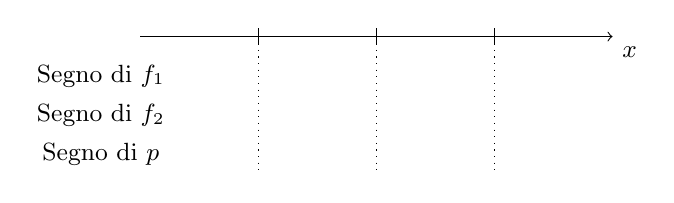
\begin{tikzpicture}[font=\small,x=10mm, y=10mm]

\draw[->] (0,0) -- (6,0) node [below right] () {$x$};

\foreach \x in {1.5,3,4.5}{
\draw(\x,3pt)--(\x,-3pt);
\begin{scope}[dotted]
\draw (\x,0) -- (\x,-1.7);
\end{scope}}
\node[] at (-.5,-0.5) {Segno di $f_1$};
\node[] at (-.5,-1) {Segno di $f_2$};
\node[] at (-.5,-1.5) {Segno di $p$};

\end{tikzpicture}

\end{center}
Otteniamo: $\IS=\left\{x\in \insR | -\frac 1 3\le x\le 0\vee x\ge 3\right\}$.
\end{esempio}

\begin{esempio}
Un numero è tale che sottraendo al suo cubo il suo triplo si ottiene un numero 
maggiore del triplo del suo quadrato aumentato di $ 4 $. Determinare l'insieme 
soluzione del problema.

La richiesta del problema implica la ricerca dell'Insieme Soluzione della 
disequazione $x^3-3x>3x^2+4$, di terzo grado nella variabile $x$. Scriviamo la 
disequazione in forma canonica, applicando i principi di equivalenza: 
$x^3-3x^2-3x-4>0$. Si tratta di una disequazione polinomiale di terzo grado.

Procediamo nella scomposizione in fattori del polinomio $p(x)=x^3-3x^2-3x-4$. 
Mediante la regola di Ruffini possiamo determinare un suo zero $x=4$ e dunque 
ottenere $p(x)=(x-4)(x^2+x+1)$.

Determiniamo il segno dei singoli fattori: primo fattore $f_1>0\to x>4$ secondo 
fattore $f_2>0\to x^2+x+1>0$ disequazione di secondo grado. Il primo 
coefficiente è positivo e il discriminante \ $\Delta =1-4=-3$ è negativo; la 
parabola volge la concavità verso l'alto e non ha zeri reali dunque il secondo 
fattore è positivo per qualunque valore reale di $x$. Costruiamo la tabella dei 
segni:
\begin{center}
 % (c) 2013 Claudio Carboncini - claudio.carboncini@gmail.com
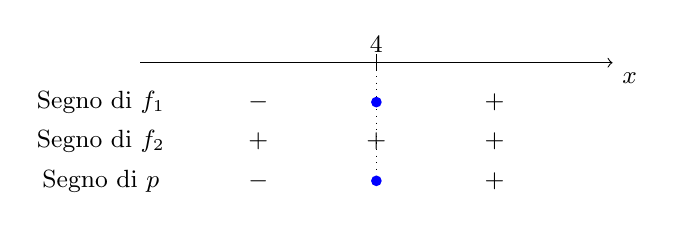
\begin{tikzpicture}[font=\small,x=10mm, y=10mm]

\draw[->] (0,0) -- (6,0) node [below right] () {$x$};

\draw(3,3pt)--(3,-3pt);
\begin{scope}[dotted]
\draw (3,0) -- (3,-1.5);
\end{scope}
\node[] at (-.5,-0.5) {Segno di $f_1$};
\node[] at (-.5,-1) {Segno di $f_2$};
\node[] at (-.5,-1.5) {Segno di $p$};
\node[above]  at (3,0) {$4$};
\node[] at (1.5,-0.5) {$-$};
\node[] at (4.5,-0.5) {$+$};
\node[] at (1.5,-1) {$+$};
\node[] at (3,-1) {$+$};
\node[] at (4.5,-1) {$+$};
\node[] at (1.5,-1.5) {$-$};
\node[] at (4.5,-1.5) {$+$};

\begin{scope}[blue,thick]
\draw[fill=blue] (3,-1.5)circle (1.5pt);
\draw[fill=blue] (3,-.5)circle (1.5pt);
\end{scope}

\end{tikzpicture}

\end{center}
$\IS=\{x\in \insR | x>4\}=(4;+\infty )$.
\end{esempio}

\begin{esempio}
Risolvere la disequazione: $64x^6-1<0$.

Il binomio al primo membro è una differenza di quadrati, quindi scomponendo si 
ottiene: $64x^6-1=(8x^3-1)(8x^3+1)=(2x-1)(4x^2+2x+1)(2x+1)(4x^2-2x+1)$.

Si tratta allora di studiare il segno dei singoli fattori: $f_1>0\to x>\frac 1 
2$ $f_2>0\to \forall x\in \insR$ $f_3>0\to x>-\frac 1 2$ $f_4>0\to \forall x\in 
\insR$ e di determinare il segno richiesto dopo aver costruito la tabella dei 
segni.
\end{esempio}

\begin{esempio}
Risolvere la disequazione: $x^4-4x^2-45>0$.

Il trinomio al primo membro è di quarto grado; sappiamo che con la sostituzione 
$x^2=t$ può essere ricondotto ad un trinomio di secondo grado la cui 
scomposizione in fattori risulta $(t-9)\cdot (t+5)$ e quindi la disequazione 
assegnata diventa: $(x^2-9)\cdot (x^2+5)>0$.

Si tratta allora di studiare il segno dei singoli fattori $f_1>0\to x<-3\vee 
x>3$ e $f_2>0\to \forall x\in \insR$ per poi determinare il segno richiesto 
dopo 
aver costruito la tabella dei segni.
\end{esempio}
% \end{exrig}
% \vspazio\ovalbox{\risolvii \ref{ese:4.32}, \ref{ese:4.33}, \ref{ese:4.34}, 
% \ref{ese:4.35}, \ref{ese:4.36}, \ref{ese:4.37}, \ref{ese:4.38}, 
% \ref{ese:4.39}, 
% \ref{ese:4.40}, \ref{ese:4.41}, \ref{ese:4.42}, \ref{ese:4.43}, \ref 
% {ese:4.44},}
% 
% \vspazio\ovalbox{\ref{ese:4.45}, \ref{ese:4.46}, \ref{ese:4.47}, 
% \ref{ese:4.48}, 
% \ref{ese:4.49}, \ref{ese:4.50}, \ref{ese:4.51}, \ref{ese:4.52}, 
% \ref{ese:4.53}, 
% \ref{ese:4.54}, \ref{ese:4.55}, \ref{ese:4.56}, \ref{ese:4.57}}

\newpage %----------------------------------------------

\section{Disequazioni fratte}
\label{sec:diseq_fratte}

Ricordiamo che una disequazione è \emph{frazionaria} o \emph{fratta} quando il 
suo denominatore contiene l'incognita. Per risolverla si può applicare la 
seguente

\begin{procedura}
Soluzione di una disequazione frazionaria:
\begin{enumeratea}
\item trasporta tutti i termini al primo membro e scrivilo sotto forma di 
 un'unica frazione: $\frac{N(x)}{D(x)} \lessgtr 0$;
% \item si determinano le Condizioni di Esistenza ponendo $D(x)\neq 0$
% \item impostiamo la disequazione nella forma $\frac{N(x)}{D(x)}\ge 0$ oppure 
% $\frac{N(x)}{D(x)}\le 0$ oppure $\frac{N(x)}{D(x)}<0$ oppure 
% $\frac{N(x)}{D(x)}>0$ a seconda del quesito posto da problema;
\item scomponi in fattori numeratore e denominatore;
\item studia il segno di ogni fattore;
\item costruisci la tabella dei segni, ricordandosi di indicare con una 
 crocetta gli zeri del denominatore;
\item applica la regola dei segni per calcolare il segno della frazione;
\item individuano gli intervalli in cui la frazione assume il segno richiesto;
\item rappresenta, con i diversi metodi visti, gli intervalli che 
 risolvono la disequazione.
\end{enumeratea}
\end{procedura}

Vediamo attraverso alcuni esempi come procedere.

 \begin{esempio}
\[\frac{2}{x-7} \ge \frac{3}{x+4}\]
\begin{itemize}
 \item Scrivere la disequazione in forma normale:
 \[\frac{2}{x-7} - \frac{3}{x+4} \ge 0 \Rightarrow 
   \frac{2 x +8 -3x +21}{(x-7)(x+4)} \ge 0 \Rightarrow
   \frac{-x +29}{(x-7)(x+4)} \ge 0\]
 \item Segno del numeratore:\\
 \begin{minipage}{.45\textwidth}
  E.A.:~$-x +29=0 \Rightarrow x=29$
 \end{minipage}
 \begin{minipage}{.25\textwidth}
  F.A.:~$y=-x +29 \rightarrow $
 \end{minipage}
 \begin{minipage}{.3\textwidth}
  % (c) 2014 Daniele Zambelli - daniele.zambelli@gmail.com

%%%
% Retta decrescente zero in 3
%%%%
 
\begin{tikzpicture}[x=1.5mm, y=1.5mm, smooth]

% (c) 2014 Daniele Zambelli - daniele.zambelli@gmail.com

%%%
% Retta decrescente con segni
%%%%
 
\coordinate (inizio) at (-10, 4);
\coordinate (zero) at (0, 0);
\coordinate (fine) at (10, -4);

% (c) 2014 Daniele Zambelli - daniele.zambelli@gmail.com

%%%
% Asse cartesiano x
%%%%

\input{lbr/assiepiani/asse10.pgf}
\node [below] at (10, 0)  {$x$};


\draw [-] [ultra thick, blue!50!black] (inizio) -- (zero);
\draw [-] [ultra thick, red!50!black] (zero) -- (fine);

\node [xshift=-25, yshift=-3, above] at (zero) {$+$};
\draw[blue, thick, fill=white] (zero) circle (2pt);
\node [xshift=25, yshift=-3, above] at (zero) {$-$};

\node [above] {$+29$};

\end{tikzpicture}

 \end{minipage}
 \item Segno del denominatore 1:\\
 \begin{minipage}{.45\textwidth}
  E.A.:~$x -7=0 \Rightarrow x=+7$
 \end{minipage}
 \begin{minipage}{.25\textwidth}
  F.A.:~$y=x -7 \rightarrow $
 \end{minipage}
 \begin{minipage}{.3\textwidth}
  % (c) 2014 Daniele Zambelli - daniele.zambelli@gmail.com

%%%
% Retta crescente zero in -2
%%%%
 
\begin{tikzpicture}[x=1.5mm, y=1.5mm, smooth]

% (c) 2014 Daniele Zambelli - daniele.zambelli@gmail.com

%%%
% Retta crescente con segni
%%%%
 
\coordinate (inizio) at (-10, -4);
\coordinate (zero) at (0, 0);
\coordinate (fine) at (10, 4);

% (c) 2014 Daniele Zambelli - daniele.zambelli@gmail.com

%%%
% Asse cartesiano x
%%%%

\input{lbr/assiepiani/asse10.pgf}
\node [below] at (10, 0)  {$x$};


\draw [-] [ultra thick, red!50!black] (inizio) -- (zero);
\draw [-] [ultra thick, blue!50!black] (zero) -- (fine);

\node [xshift=-25, yshift=-3, above] at (zero) {$-$};
\draw[blue, thick, fill=white] (zero) circle (2pt);
\node [xshift=25, yshift=-3, above] at (zero) {$+$};

\node [above] {$+7$};

\end{tikzpicture}

 \end{minipage}
 \item Segno del denominatore 2:\\
 \begin{minipage}{.45\textwidth}
  E.A.:~$x +4=0 \Rightarrow x=-4$
 \end{minipage}
 \begin{minipage}{.25\textwidth}
  F.A.:~$y=x +4 \rightarrow $
 \end{minipage}
 \begin{minipage}{.3\textwidth}
  % (c) 2014 Daniele Zambelli - daniele.zambelli@gmail.com

%%%
% Retta crescente zero in -2
%%%%
 
\begin{tikzpicture}[x=1.5mm, y=1.5mm, smooth]

% (c) 2014 Daniele Zambelli - daniele.zambelli@gmail.com

%%%
% Retta crescente con segni
%%%%
 
\coordinate (inizio) at (-10, -4);
\coordinate (zero) at (0, 0);
\coordinate (fine) at (10, 4);

% (c) 2014 Daniele Zambelli - daniele.zambelli@gmail.com

%%%
% Asse cartesiano x
%%%%

\input{lbr/assiepiani/asse10.pgf}
\node [below] at (10, 0)  {$x$};


\draw [-] [ultra thick, red!50!black] (inizio) -- (zero);
\draw [-] [ultra thick, blue!50!black] (zero) -- (fine);

\node [xshift=-25, yshift=-3, above] at (zero) {$-$};
\draw[blue, thick, fill=white] (zero) circle (2pt);
\node [xshift=25, yshift=-3, above] at (zero) {$+$};

\node [above] {$-4$};

\end{tikzpicture}

 \end{minipage}
 \item Con la regola dei segni calcolo il segno della frazione 
  % (c) 2014 Daniele Zambelli - daniele.zambelli@gmail.com

%%%
% Studio dei segni di una frazione
%%%%
 
\begin{tikzpicture}[x=2.5mm, y=5mm, smooth]

\coordinate (a_top) at (-5, 1);
\coordinate (a_bottom) at (-5, -3);
\coordinate (b_top) at (0, 1);
\coordinate (b_bottom) at (0, -3);
\coordinate (c_top) at (5, 1);
\coordinate (c_bottom) at (5, -3);

% (c) 2014 Daniele Zambelli - daniele.zambelli@gmail.com

%%%
% Grafo per il calcolo del segno con tre assi
%%%%
 
% (c) 2014 Daniele Zambelli - daniele.zambelli@gmail.com

%%%
% Asse cartesiano x
%%%%

\input{lbr/assiepiani/asse10.pgf}
\node [below] at (10, 0)  {$x$};

\begin{scope}[yshift= -.5cm]
  % (c) 2014 Daniele Zambelli - daniele.zambelli@gmail.com

%%%
% Asse cartesiano x
%%%%

\input{lbr/assiepiani/asse10.pgf}
\node [below] at (10, 0)  {$x$};

  \begin{scope}[yshift= -.5cm]
    % (c) 2014 Daniele Zambelli - daniele.zambelli@gmail.com

%%%
% Asse cartesiano x
%%%%

\input{lbr/assiepiani/asse10.pgf}
\node [below] at (10, 0)  {$x$};

    \begin{scope}[yshift= -.5cm]
      % (c) 2014 Daniele Zambelli - daniele.zambelli@gmail.com

%%%
% Asse cartesiano x
%%%%

\input{lbr/assiepiani/asse10.pgf}
\node [below] at (10, 0)  {$x$};

    \end{scope}
  \end{scope}
\end{scope}

\draw [-] [] (a_top) -- (a_bottom);
\draw [-] [] (b_top) -- (b_bottom);
\draw [-] [] (c_top) -- (c_bottom);

\node [above] at (-5, 1) {$-4$};
\node [above] at (0, 1) {$+7$};
\node [above] at (5, 1) {$+29$};

\node [above left] at (-10, 0) {$-x+29$};
\node [above] at (-7.5, 0) {$+$};
\node [above] at (-2.5, 0) {$+$};
\node [above] at (2.5, 0) {$+$};
\draw (5, .5) circle (3pt);
\node [above] at (7.5, 0) {$-$};

\node [above left] at (-10, -1) {$x-7$};
\node [above] at (-7.5, -1) {$-$};
\node [above] at (-2.5, -1) {$-$};
\draw (0 -.4, -0.5 -.2) -- (0 +.4, -0.5 +.2) 
      (0 -.4, -0.5 +.2) -- (0 +.4, -0.5 -.2);
\node [above] at (2.5, -1) {$+$};
\node [above] at (7.5, -1) {$+$};

\node [above left] at (-10, -2) {$x+4$};
\node [above] at (-7.5, -2) {$-$};
\draw (-5 -.4, -1.5 -.2) -- (-5 +.4, -1.5 +.2) 
      (-5 -.4, -1.5 +.2) -- (-5 +.4, -1.5 -.2);
\node [above] at (-2.5, -2) {$+$};
\node [above] at (2.5, -2) {$+$};
\node [above] at (7.5, -2) {$+$};

\node [above left] at (-10, -3.15) {$F(x)$};
\node [above] at (-7.5, -3) {$+$};
\draw (-5 -.4, -2.5 -.2) -- (-5 +.4, -2.5 +.2) 
      (-5 -.4, -2.5 +.2) -- (-5 +.4, -2.5 -.2);
\node [above] at (-2.5, -3) {$-$};
\draw (0 -.4, -2.5 -.2) -- (0 +.4, -2.5 +.2) 
      (0 -.4, -2.5 +.2) -- (0 +.4, -2.5 -.2);
\node [above] at (2.5, -3) {$+$};
\draw (5, -2.5) circle (3pt);
\node [above] at (7.5, -3) {$-$};

\end{tikzpicture}
 
 \item Quindi i valori di~$x$ che rendono vera la disequazione, cioè i valori
  che rendono~$f(x)$ negativo, sono quelli 
  che si trovano a sinistra di~$-2$ oppure che si trovano a destra di~$+3$. 
 \subitem 
  \begin{minipage}{.35\textwidth}
   rappresentazione grafica: 
  \end{minipage}
  \begin{minipage}{.30\textwidth}
   % (c) 2014 Daniele Zambelli - daniele.zambelli@gmail.com

%%%
% Valori x < -4  or  7 < x <= 29
%%%%
 
\begin{tikzpicture}[x=1.5mm, y=1.5mm, smooth]

% \clip (-7.5, -5.5) rectangle (10.9, 10.9);

\coordinate (m_i) at (-10, 0);
\coordinate (a) at (-5, 0);
\coordinate (b) at (0, 0);
\coordinate (c) at (5, 0);
\coordinate (p_i) at (10, 0);

% (c) 2014 Daniele Zambelli - daniele.zambelli@gmail.com

%%%
% Asse cartesiano x
%%%%

% (c) 2014 Daniele Zambelli - daniele.zambelli@gmail.com

%%%
% Asse cartesiano generico
%%%%

\draw [-{Stealth[length=2mm, open, round]}] (-10, 0) -- (10, 0);

\node [below] at (10, 0)  {$x$};


\begin{scope}[blue,thick]
\draw [-,decorate,decoration=snake] (m_i) -- (a);
% \draw[fill=white] (a) circle (2pt) node [above] {$-3$};
\draw[fill=white] (a) circle (2pt) node [above] {$-4$};
% \draw [-,decorate,decoration=snake] (b) -- (c);
\draw[fill=white] (b) circle (2pt) node [above] {$+7$};
\draw [decorate,decoration=snake] (b) -- (c);
\draw[fill] (c) circle (2pt) node [above] {$+29$};
\end{scope}

\end{tikzpicture}

  \end{minipage}
 \subitem rappresentazione con i 
  predicati:~$x < -4 \quad \lor \quad +7 < x \le 29$ 
 \subitem rappresentazione con le 
  parentesi:~$]-\infty;~-4[ \quad \cup \quad ]+7;~+\infty[$. 
\end{itemize}
 \end{esempio}

% \begin{exrig}
\begin{esempio}
Data l'espressione $E=\frac 4{4x^2-1}+\frac 1{2x+1}+\frac x{1-2x}$ 
determinarne, 
al variare di $x$ in $\insR$, il segno.

\emph{Osservazioni preliminari}
\begin{itemize*}
\item L'espressione assegnata è frazionaria, quindi lo studio del segno deve 
essere circoscritto ai valori di $x$ del Dominio dell'espressione stessa;
\item studiare il segno di una espressione letterale significa stabilire in 
quale insieme si trovano i valori della variabile che la rendono positiva, 
negativa, nulla;
\item ogni espressione contenente operazioni tra frazioni algebriche ha in 
generale come risultato una frazione algebrica.
\end{itemize*}

\emph{Strategia risolutiva}
\begin{enumeratea}
\item determiniamo il risultato dell'operazione assegnata: 
$E=\frac{-2x^2+x+3}{(2x+1)\cdot (2x-1)}$
\item determiniamo il dominio: $\CE\, 2x+1\neq 0\wedge 2x-1\neq 0\to 
D=\insR-\left\{-\frac 1 2,\frac 1 2\right\}$
\item impostiamo la disequazione: $\frac{-2x^2+x+3}{(2x+1)\cdot (2x-1)}\ge 0$ 
che ci permetterà di rispondere al quesito posto dal problema;
\item studiamo il segno di numeratore e denominatore:
 \begin{itemize*}
\item segno $N: -2x^2+x+3\ge 0$ disequazione di secondo grado, quindi 
dall'equazione associata $-2x^2+x+3=0$, calcoliamo il discriminante: $\Delta 
=1+24=25$, positivo per cui si hanno due soluzioni reali distinte; la parabola 
$y=-2x^2+x+3$ ha concavità verso il basso per cui essendo $x_1=-1$ e $x_2=\frac 
3 2$ si ha $N\ge 0$ per $-1\le x\le \frac 3 2$
\item segno $D$: il denominatore è composto da due fattori di primo grado, 
quindi $d_1>0$ per $x>-\frac 1 2$ e $d_2>0$ per $x>\frac 1 2$
 \end{itemize*}
\item costruiamo la tabella dei segni:
\begin{center}
 % (c) 2013 Claudio Carboncini - claudio.carboncini@gmail.com
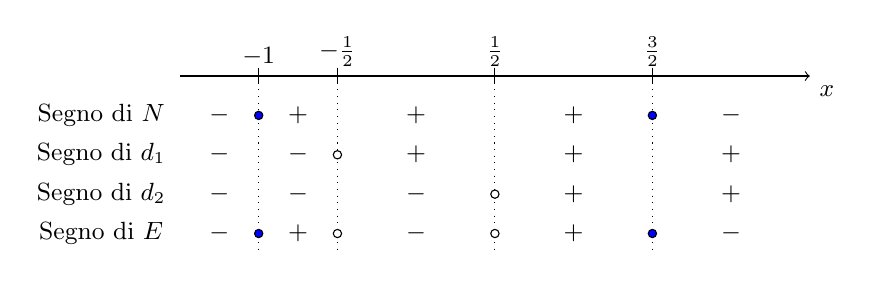
\begin{tikzpicture}[font=\small,x=10mm, y=10mm]

\draw[->] (0,0) -- (8,0) node [below right] () {$x$};

\foreach \x in {1,2,4,6}{
\draw(\x,3pt)--(\x,-3pt);
\begin{scope}[dotted]
\draw (\x,0) -- (\x,-2.2);
\end{scope}}
\node[] at (-1,-0.5) {Segno di $N$};
\draw[fill=blue] (1,-.5)circle (1.5pt);
\draw[fill=blue] (6,-.5)circle (1.5pt);
\node[] at (-1,-1) {Segno di $d_1$};
\draw[fill=white] (2,-1)circle (1.5pt);
\node[] at (-1,-1.5) {Segno di $d_2$};
\draw[fill=white] (4,-1.5)circle (1.5pt);
\node[] at (-1,-2) {Segno di $E$};
\draw[fill=blue] (1,-2)circle (1.5pt);
\draw[fill=blue] (6,-2)circle (1.5pt);
\draw[fill=white] (2,-2)circle (1.5pt);
\draw[fill=white] (4,-2)circle (1.5pt);
\node[above]  at (1,0) {$-1$};
\node[above]  at (2,0) {$-{\frac{1}{2}}$};
\node[above]  at (4,0) {${\frac{1}{2}}$};
\node[above]  at (6,0) {${\frac{3}{2}}$};
\node[] at (.5,-0.5) {$-$};
\node[] at (1.5,-0.5) {$+$};
\node[] at (3,-0.5) {$+$};
\node[] at (5,-0.5) {$+$};
\node[] at (7,-0.5) {$-$};
\node[] at (.5,-1) {$-$};
\node[] at (1.5,-1) {$-$};
\node[] at (3,-1) {$+$};
\node[] at (5,-1) {$+$};
\node[] at (7,-1) {$+$};
\node[] at (.5,-1.5) {$-$};
\node[] at (1.5,-1.5) {$-$};
\node[] at (3,-1.5) {$-$};
\node[] at (5,-1.5) {$+$};
\node[] at (7,-1.5) {$+$};
\node[] at (.5,-2) {$-$};
\node[] at (1.5,-2) {$+$};
\node[] at (3,-2) {$-$};
\node[] at (5,-2) {$+$};
\node[] at (7,-2) {$-$};

\end{tikzpicture}

\end{center}
\item dalla tabella dei segni possiamo ottenere la risposta al problema posto:
\begin{itemize*}
\item l'espressione $E$ si annulla per $x=-1\vee x=\frac 3 2$
\item l'espressione $E$ è positiva per $x\in A=\left\{x\in \insR | -1<x<-\frac 
1 
2\vee \frac 1 2<x<\frac 3 2\right\}$
\item l'espressione $E$ è negativa per $x\in B=\left\{x\in \insR | x<-1\vee 
-\frac 1 2<x<\frac 1 2\vee x>\frac 3 2\right\}$.
\end{itemize*}
\end{enumeratea}
\end{esempio}

\begin{esempio}
Determiniamo l'Insieme Soluzione della disequazione fratta: $3-\frac 1{2x+1}\ge 
\frac 1{1-x}$.
\begin{enumeratea}
\item Trasportiamo al primo membro la frazione del secondo membro $E=3-\frac 
1{2x+1}-\frac 1{1-x}$ ed eseguiamo i calcoli ottenendo: 
$E=\frac{-6x^2+2x+1}{(2x+1)\cdot (1-x)}$
\item determiniamo il dominio: $\CE \;2x+1\neq 0\wedge 1-x\neq 0\to 
D=\insR-\left\{-\frac 1 2,1\right\}$
\item impostiamo la disequazione: \ $\frac{-6x^2+2x+1}{(2x+1)\cdot (1-x)}\ge 0$ 
che ci permetterà di rispondere al quesito posto dal problema;
\item studiamo il segno del numeratore e del denominatore:
\begin{itemize*}
\item segno N: $-6x^2+2x+1\ge 0$ disequazione di secondo grado, quindi scritta 
l'equazione associata $-6x^2+2x+1=0$, calcoliamone il discriminante: 
$\frac{\Delta } 4=7$, positivo per cui si hanno due soluzioni 
$x_{1,2}=\frac{1\pm \sqrt 7} 6$ essendo il primo coefficiente negativo si ha 
$N\ge 0$ per $\frac{1-\sqrt 7} 6\le x\le \frac{1+\sqrt 7} 6$
\item segno D: $-2x^2+x+1>0$ disequazione di secondo grado; il denominatore ha 
due zeri reali $x=-\frac 1 2$ e $x_2=1$, il primo coefficiente è negativo, 
pertanto $D>0$ per $-\frac 1 2<x<1$ che rispetta le C.E.: $x_1\neq -\frac 1 
2\wedge x_2\neq 1$
\end{itemize*}
\item compiliamo la tabella dei segni:
\begin{center}
 % (c) 2013 Claudio Carboncini - claudio.carboncini@gmail.com
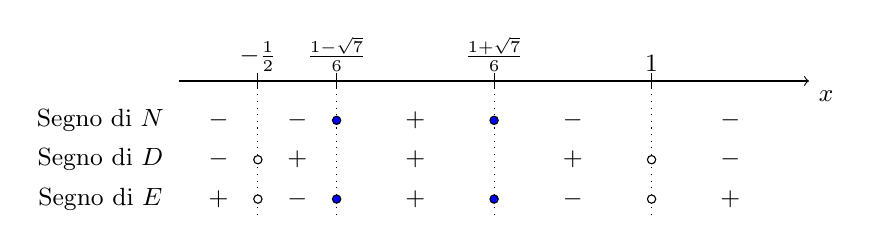
\begin{tikzpicture}[font=\small,x=10mm, y=10mm]

\draw[->] (0,0) -- (8,0) node [below right] () {$x$};

\foreach \x in {1,2,4,6}{
\draw(\x,3pt)--(\x,-3pt);
\begin{scope}[dotted]
\draw (\x,0) -- (\x,-1.7);
\end{scope}}

\node[] at (-1,-0.5) {Segno di $N$};
\draw[fill=blue] (2,-.5)circle (1.5pt);
\draw[fill=blue] (4,-.5)circle (1.5pt);
\node[] at (-1,-1) {Segno di $D$};
\draw[fill=white] (1,-1)circle (1.5pt);
\draw[fill=white] (6,-1)circle (1.5pt);
\node[] at (-1,-1.5) {Segno di $E$};
\draw[fill=blue] (2,-1.5)circle (1.5pt);
\draw[fill=blue] (4,-1.5)circle (1.5pt);
\draw[fill=white] (1,-1.5)circle (1.5pt);
\draw[fill=white] (6,-1.5)circle (1.5pt);
\node[above]  at (1,0) {$-{\frac{1}{2}}$};
\node[above]  at (2,0) {${\frac{1-\sqrt{7}}{6}}$};
\node[above]  at (4,0) {${\frac{1+\sqrt{7}}{6}}$};
\node[above]  at (6,0) {$1$};
\node[] at (.5,-0.5) {$-$};
\node[] at (1.5,-0.5) {$-$};
\node[] at (3,-0.5) {$+$};
\node[] at (5,-0.5) {$-$};
\node[] at (7,-0.5) {$-$};
\node[] at (.5,-1) {$-$};
\node[] at (1.5,-1) {$+$};
\node[] at (3,-1) {$+$};
\node[] at (5,-1) {$+$};
\node[] at (7,-1) {$-$};
\node[] at (.5,-1.5) {$+$};
\node[] at (1.5,-1.5) {$-$};
\node[] at (3,-1.5) {$+$};
\node[] at (5,-1.5) {$-$};
\node[] at (7,-1.5) {$+$};

\end{tikzpicture}

\end{center}
\item determiniamo l'insieme soluzione: $\IS=\left\{x\in \insR | x<-\frac 1 
2\vee \frac{1-\sqrt 7} 6\le x\le \frac{1+\sqrt 7} 6\vee x>1\right\}$.
\end{enumeratea}
\end{esempio}
% \end{exrig}

% \vspazio\ovalbox{\risolvii \ref{ese:4.58}, \ref{ese:4.59}, \ref{ese:4.60}, 
% \ref{ese:4.61}, \ref{ese:4.62}, \ref{ese:4.63}, \ref{ese:4.64}, 
% \ref{ese:4.65}, 
% \ref{ese:4.66}, \ref{ese:4.67}, \ref{ese:4.68}, \ref{ese:4.69}, \ref 
% {ese:4.70},}
% 
% \vspazio\ovalbox{\ref{ese:4.71}, \ref{ese:4.72}, \ref{ese:4.47}, 
% \ref{ese:4.73}, 
% \ref{ese:4.74}}

\section{Sistemi di disequazioni}
\label{sec:diseq_sistemi}

Ricordiamo che risolvere un sistema di disequazioni significa trovare l'insieme 
dei numeri reali che sono le soluzioni comuni alle disequazioni che lo 
compongono. Indicate con $d_{1}, d_{2}, \ldots, d_n$ le disequazioni che 
formano 
il sistema e $\IS_{1}, \IS_{2}, \ldots,\IS_n$ i rispettivi insieme soluzione, 
la 
soluzione del sistema indicata con $\IS$ è data da $\IS=\IS_1\cap 
\IS_{2,}\ldots 
\cap \IS_n$.

\begin{problema}
Nell'equazione $x^2-(k-3)x+k^2-3k+1=0$, determinare per quali valori del 
parametro $ k $ si ottengono soluzioni reali e concordi.
\end{problema}
Abbiamo già affrontato un \ problema di questo tipo discutendo le equazioni 
parametriche di secondo grado e dunque sappiamo che la richiesta del problema 
esige che il discriminante $(\Delta )$ sia non negativo affinché le soluzioni 
siano reali e che il prodotto delle stesse sia positivo. Pertanto il problema è 
formalizzato con un sistema di disequazioni: $\left\{\begin{array}{l}{\Delta 
\ge 
0}\\{\frac c a>0}\end{array}\right. \to 
\left\{\begin{array}{l}{k^2-6k+9-4k^2+12k-4\ge 
0}\\{k^2-3k+1>0}\end{array}\right.$.

Risolviamo separatamente le due disequazioni del sistema; indicati con $\IS_1$ 
e 
$\IS_2$ rispettivamente gli insiemi soluzione della prima e della seconda 
disequazione, l'insieme soluzione del sistema è dato da $\IS=\IS_1\cap \IS_2$ 
(insieme intersezione degli insiemi soluzione delle due disequazioni).
\begin{itemize*}
\item $d_1$: $-3k^2+6k+5\ge 0$ disequazione di secondo grado avente primo 
coefficiente negativo e $\frac{\Delta } 4=24$ positivo; la parabola 
$y=-3k^2+6k+5\ge 0$ ha concavità verso il basso e discriminante positivo, per 
cui essendo $x_1=\frac{3-2\sqrt 6} 3\vee x_2=\frac{3+2\sqrt 6} 3$ si ottiene 
$\IS_1=\left\{x\in \insR | \frac{3-2\sqrt 6} 3\le x\le \frac{3+2\sqrt 6} 
3\right\}$.
\item $d_2$: $k^2-3k+1>0$ disequazione di secondo grado avente il primo 
coefficiente positivo e $\Delta =5$ positivo; la parabola $y=k^2-3k+1>0$ ha 
concavità verso l'alto e discriminante positivo, quindi $x_1=\frac{3-\sqrt 5} 
2\vee x_2=\frac{3+\sqrt 5} 2$ e
$\IS_2=~\left\{x\in \insR | x<\frac{3-\sqrt 5} 2\vee x>\frac{3+\sqrt 5} 
2\right\}$.
\end{itemize*}
Per determinare l'Insieme Soluzione del sistema rappresentiamo in un grafico 
gli 
insiemi soluzioni delle disequazioni risolte e visualizziamo l'insieme formato 
dai valori che soddisfano contemporaneamente sia l'una che l'altra: sull'asse 
reale depositiamo i valori numerici trovati e rappresentiamo su righe distinte 
i 
due insiemi soluzione: gli intervalli in cui cadono soluzioni della prima e 
della seconda disequazione rappresentano l'Insieme Soluzione del sistema.
\begin{center}
 % (c) 2013 Claudio Carboncini - claudio.carboncini@gmail.com
\begin{tikzpicture}[font=\small,x=10mm, y=10mm]

\draw[->] (0,0) -- (8,0) node [below right] () {$r$};

\foreach \x in {2,3.5,5,6.5}{
\draw(\x,3pt)--(\x,-3pt);
\begin{scope}[dotted]
\draw (\x,0) -- (\x,-2);
\draw (0,-.5) -- (2,-.5);
\draw (6.5,-.5) -- (8,-.5);
\draw (3.5,-1) -- (5,-1);
\draw (0,-1.5) -- (2,-1.5);
\draw (3.5,-1.5) -- (5,-1.5);
\draw (6.5,-1.5) -- (8,-1.5);
\end{scope}}

\node[above]  at (2,0) {$\frac{3-2 \sqrt{6}}{3}$};
\node[above]  at (3.5,0) {$\frac{3- \sqrt{5}}{2}$};
\node[above]  at (5,0) {$\frac{3+ \sqrt{5}}{2}$};
\node[above]  at (6.5,0) {$\frac{3+2 \sqrt{6}}{3}$};
\pattern[pattern= north east lines, pattern color=red] (2,-2) rectangle (3.5,-1.5);
\pattern[pattern= north east lines, pattern color=red] (5,-2) rectangle (6.5,-1.5);

\node[] () at (-.5,-.5) {$\IS_{1}$};
\node[] () at (-.5,-1) {$\IS_{2}$};
\node[] () at (-.5,-1.75) {$\IS$};

\begin{scope}[blue,thick]
\draw (2,-.5) -- (6.5,-.5);
\draw (0,-1) -- (3.5,-1);
\draw (5,-1) -- (8,-1);
\draw (2,-1.5) -- (3.5,-1.5);
\draw (5,-1.5) -- (6.5,-1.5);

\draw[fill=blue] (2,-.5)circle (1.5pt);
\draw[fill=blue] (6.5,-.5)circle (1.5pt);
\draw[fill=white] (3.5,-1)circle (1.5pt);
\draw[fill=white] (5,-1)circle (1.5pt);
\draw[fill=blue] (2,-1.5)circle (1.5pt);
\draw[fill=blue] (6.5,-1.5)circle (1.5pt);
\draw[fill=white] (3.5,-1.5)circle (1.5pt);
\draw[fill=white] (5,-1.5)circle (1.5pt);

\end{scope}

\end{tikzpicture}

\end{center}

$\IS_1=\left\{x\in \insR\left|\frac{3-2\sqrt 6} 3\le x<\frac{3-\sqrt 5} 2\vee 
\frac{3+\sqrt 5} 2<x\le \frac{3+2\sqrt 6} 3\right.\right\}$

o scritto utilizzando gli intervalli: 

$\left.\left[\frac{3-2\sqrt 6} 3;\frac{3-\sqrt 5} 
2\right.\right[ \cup \left.\left]\frac{3+\sqrt 5} 2;\frac{3+2\sqrt 6} 
3\right.\right]$.

\begin{problema}
Risolvere il seguente sistema di disequazioni: $ 
\left\{\begin{array}{l}2x^3-9x^2+10x-3\le 0\\ \frac{x^2+x+1}{\ x^3-x}\ge 0 
\\3-4x<0 \end{array}\right.$.
\end{problema}
Il sistema è formato da tre disequazioni; risolviamo separatamente ciascuna 
disequazione:

\begin{itemize*}
\item $d_1$: $2x^3-9x^2+10x-3\le 0$ di terzo grado, scomponiamo in fattori. 
$x=1$ è uno zero del polinomio quindi con la regola di Ruffini otteniamo $d_1$: 
$(x-1)\cdot (2x^2-7x+3)\le 0$. L'equazione di secondo grado $2x^2-7x+3=0$ ha 
soluzioni reali $x_1=\frac 1 2\vee x=3$. Si tratta allora di studiare il segno 
dei singoli fattori e di determinare il segno richiesto dopo aver costruito la 
tabella dei segni:
\begin{center}
 % (c) 2013 Claudio Carboncini - claudio.carboncini@gmail.com
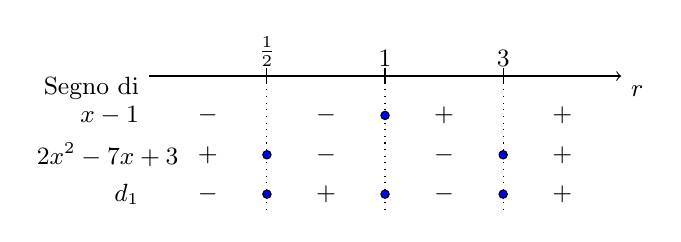
\begin{tikzpicture}[font=\small,x=10mm, y=10mm]

\draw[->] (0,0) -- (6,0) node [below right] () {$r$};

\foreach \x in {1.5,3,4.5}{
\draw(\x,3pt)--(\x,-3pt);
\begin{scope}[dotted]
\draw (\x,0) -- (\x,-1.7);
\end{scope}}

\node[left] at (0,-0.15) {Segno di};
\node[left] at (0,-0.5) {$x-1$};
\node[left] at (.5,-1) {$2x^2-7x+3$};
\node[left] at (0,-1.5) {$d_1$};
\node[above]  at (1.5,0) {$\frac{1}{2}$};
\node[above]  at (3,0) {$1$};
\node[above]  at (4.5,0) {$3$};
\node[] at (.75,-0.5) {$-$};
\node[] at (2.25,-0.5) {$-$};
\node[] at (3.75,-0.5) {$+$};
\node[] at (5.25,-0.5) {$+$};
\node[] at (.75,-1) {$+$};
\node[] at (2.25,-1) {$-$};
\node[] at (3.75,-1) {$-$};
\node[] at (5.25,-1) {$+$};
\node[] at (.75,-1.5) {$-$};
\node[] at (2.25,-1.5) {$+$};
\node[] at (3.75,-1.5) {$-$};
\node[] at (5.25,-1.5) {$+$};

\draw[fill=blue] (3,-.5)circle (1.5pt);
\draw[fill=blue] (1.5,-1)circle (1.5pt);
\draw[fill=blue] (4.5,-1)circle (1.5pt);
\draw[fill=blue] (3,-1.5)circle (1.5pt);
\draw[fill=blue] (1.5,-1.5)circle (1.5pt);
\draw[fill=blue] (4.5,-1.5)circle (1.5pt);

\end{tikzpicture}

\end{center}
L'insieme soluzione, tenendo conto che cerchiamo i valori per i quali $d_1$ 
risulta minore o uguale a $0$ è $\IS_1=\left\{x\in \insR | x\le\frac 1 2\vee 
1\le x\le 3\right\}$.

\item $d_2$: $\frac{x^2+x+1}{x^3-x}\ge 0$ è una disequazione fratta, per prima 
cosa scomponiamo in fattori il denominatore: $\frac{x^2+x+1}{x(x^2-1)}\ge 0$.
Studiamo poi il segno dei singoli fattori o divisori, tenendo conto che 
$x^2+x+1=0$ ha $\Delta <0$, per cui $x^2+x+1$ è sempre positivo.
\begin{center}
 % (c) 2013 Claudio Carboncini - claudio.carboncini@gmail.com
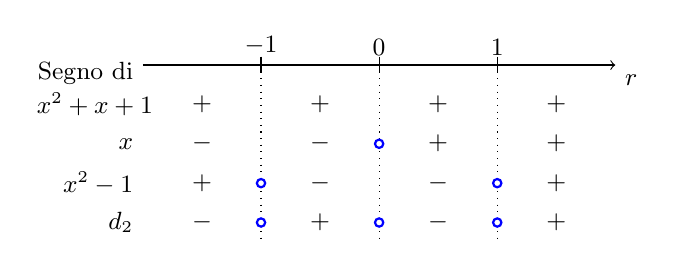
\begin{tikzpicture}[font=\small,x=10mm, y=10mm]

\draw[->] (0,0) -- (6,0) node [below right] () {$r$};

\foreach \x in {1.5,3,4.5}{
\draw(\x,3pt)--(\x,-3pt);
\begin{scope}[dotted]
\draw (\x,0) -- (\x,-2.2);
\end{scope}}

\node[left] at (0,-0.1) {Segno di};
\node[left] at (.25,-0.5) {$x^2+x+1$};
\node[left] at (0,-1) {$x$};
\node[left] at (0,-1.5) {$x^2-1$};
\node[left] at (0,-2) {$d_2$};
\node[above]  at (1.5,0) {$-1$};
\node[above]  at (3,0) {$0$};
\node[above]  at (4.5,0) {$1$};
\node[] at (.75,-0.5) {$+$};
\node[] at (2.25,-0.5) {$+$};
\node[] at (3.75,-0.5) {$+$};
\node[] at (5.25,-0.5) {$+$};
\node[] at (.75,-1) {$-$};
\node[] at (2.25,-1) {$-$};
\node[] at (3.75,-1) {$+$};
\node[] at (5.25,-1) {$+$};
\node[] at (.75,-1.5) {$+$};
\node[] at (2.25,-1.5) {$-$};
\node[] at (3.75,-1.5) {$-$};
\node[] at (5.25,-1.5) {$+$};
\node[] at (.75,-2) {$-$};
\node[] at (2.25,-2) {$+$};
\node[] at (3.75,-2) {$-$};
\node[] at (5.25,-2) {$+$};

\begin{scope}[blue,thick]
\draw[fill=white] (3,-1)circle (1.5pt);
\draw[fill=white] (1.5,-1.5)circle (1.5pt);
\draw[fill=white] (4.5,-1.5)circle (1.5pt);
\draw[fill=white] (3,-2)circle (1.5pt);
\draw[fill=white] (1.5,-2)circle (1.5pt);
\draw[fill=white] (4.5,-2)circle (1.5pt);
\end{scope}

\end{tikzpicture}

\end{center}
L'insieme soluzione, per $d_2\ge 0$ è $\IS_2=\left\{x\in \insR | -1<x<0\vee 
x>1\right\}$.
\item $d_3:3-4x<0$ è di primo grado per cui l'insieme soluzione è 
$\IS_3=\left\{x\in \insR | x>\frac 3 4\right\}$.
\end{itemize*}
Ricordiamo che la ricerca dell'Insieme Soluzione del sistema si effettua 
determinando l'insieme $\IS_1\cap \IS_2\cap \IS_3$ individuabile attraverso il 
grafico:
\begin{center}
 % (c) 2012 Dimitrios Vrettos - d.vrettos@gmail.com
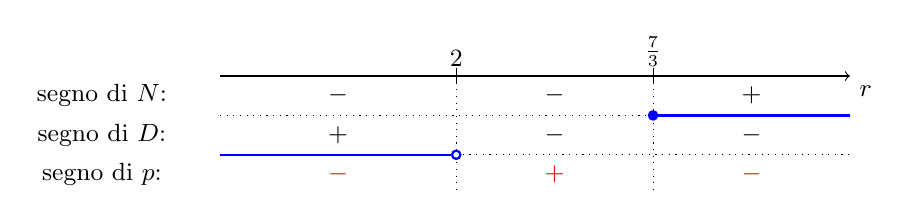
\begin{tikzpicture}[font=\small,x=10mm, y=10mm]

\draw[->] (0,0) -- (8,0) node [below right] () {$r$};

\foreach \x in {3,5.5}{
\draw(\x,3pt)--(\x,-3pt);
\begin{scope}[dotted]
\draw (\x,0) -- (\x,-1.5);
\draw (0,-.5) -- (5.5,-.5);
\draw (3,-1) -- (8,-1);
\end{scope}}

\node[above]  at (3,0) {$2$};
\node[above]  at (5.5,0) {$\frac{7}{3}$};

\begin{scope}[blue,thick]
\draw (5.5,-.5) -- (8,-.5);
\draw (3,-1) -- (0,-1);

\draw[fill=blue] (5.5,-.5)circle (1.5pt);
\draw[fill=white] (3,-1)circle (1.5pt);
\end{scope}

\foreach \x in {-1.5}{
\node  at (\x,-.25) {segno di $N$:};
\node  at (\x,-.75) {segno di $D$:};
\node  at (\x,-1.25) {segno di $p$:};
}
\foreach \z in {1.5,4.25}
\node  at (\z,-.25) {$-$};

\foreach \zi in {4.25,6.75}
\node  at (\zi,-.75) {$-$};

\node  at (6.75,-.25) {$+$};
\node  at (1.5,-.75) {$+$};

\begin{scope}[red]
\foreach \y in {-1.25}{
\foreach \ziv in {4.25}
	\node at (\ziv,\y) {$+$};
\foreach \zv in {1.5,6.75}
\node at (\zv,\y) {$-$};
}
\end{scope}
\end{tikzpicture}
\end{center}
Il sistema è quindi verificato per $1<x\le 3$  cioè: $ \left] 1;~3 \right]$.

% \vspazio\ovalbox{\risolvii \ref{ese:4.75}, \ref{ese:4.76}, \ref{ese:4.77}, 
% \ref{ese:4.78}, \ref{ese:4.79}, \ref{ese:4.80}, \ref{ese:4.81}, 
% \ref{ese:4.82}, 
% \ref{ese:4.83}}
